%%%%%%%%%%%%%%%%%%%%%%%%%%%%%%%%%%%%%%%%%%%%%%%%%%%%%%%%%%%%%%%%%%%%%%%%%%%%
% AGUtmpl.tex: this template file is for articles formatted with LaTeX2e,
% Modified July 2011
%
% This template includes commands and instructions
% given in the order necessary to produce a final output that will
% satisfy AGU requirements.
%
% PLEASE DO NOT USE YOUR OWN MACROS
% DO NOT USE \newcommand, \defcommand, or \renewcommand.
%
% FOR FIGURES, DO NOT USE \psfrag or \subfigure.
%
%%%%%%%%%%%%%%%%%%%%%%%%%%%%%%%%%%%%%%%%%%%%%%%%%%%%%%%%%%%%%%%%%%%%%%%%%%%%
%
% All questions should be e-mailed to latex@agu.org.
%
%%%%%%%%%%%%%%%%%%%%%%%%%%%%%%%%%%%%%%%%%%%%%%%%%%%%%%%%%%%%%%%%%%%%%%%%%%%%
%
% Step 1: Set the \documentclass
%
% There are two options for article format: two column (default)
% and draft.
%
% PLEASE USE THE DRAFT OPTION TO SUBMIT YOUR PAPERS.
% The draft option produces double spaced output.
%
% Choose the journal abbreviation for the journal you are
% submitting to:

% jgrga JOURNAL OF GEOPHYSICAL RESEARCH
% gbc   GLOBAL BIOCHEMICAL CYCLES
% grl   GEOPHYSICAL RESEARCH LETTERS
% pal   PALEOCEANOGRAPHY
% ras   RADIO SCIENCE
% rog   REVIEWS OF GEOPHYSICS
% tec   TECTONICS
% wrr   WATER RESOURCES RESEARCH
% gc    GEOCHEMISTRY, GEOPHYSICS, GEOSYSTEMS
% sw    SPACE WEATHER

% (If you are submitting to a journal other than jgrga,
% substitute the initials of the journal for "jgrga" below.)

\documentclass[draft,jgrga]{AGUTeX}

%%%%%%%%%%%%%%%%%%%%%%%%%%%%%%%%%%%%%%%%%%%%%%%%%%%%%%%%%%%%%%%%%%%%%%%%%
% OPTIONAL:
% To produce a two-columned version:
% \documentclass[grl]{AGUTeX}

% Two-columned format can be used to estimate the number of pages
% for the final published PDF.

% PLEASE USE THE DRAFT OPTION TO SUBMIT YOUR PAPERS.
%%%%%%%%%%%%%%%%%%%%%%%%%%%%%%%%%%%%%%%%%%%%%%%%%%%%%%%%%%%%%%%%%%%%%%%%%
% OPTIONAL:
% To create numbered lines:

% If you don't already have lineno.sty, you can download it from
% http://www.ctan.org/tex-archive/macros/latex/contrib/ednotes/
% (or search the internet for lineno.sty ctan), available at TeX
%Archive Network (CTAN).
% Take care that you always use the latest version.

% To activate the commands, uncomment \usepackage{lineno}
% and \linenumbers*[1]command, below:
% To activate the commands, uncomment \usepackage{lineno}
% and \linenumbers*[1]command, below:
\usepackage{amsmath, amsthm, amssymb}
 \usepackage{lineno}
 \linenumbers*[1]

 %\usepackage{lineno}
 %\linenumbers*[1]

%  To add line numbers to lines with equations:

%  \begin{linenomath*}
%  \begin{equation}
%  \end{equation}
%  \end{linenomath*}
%%%%%%%%%%%%%%%%%%%%%%%%%%%%%%%%%%%%%%%%%%%%%%%%%%%%%%%%%%%%%%%%%%%%%%%%%
% Figures and Tables
%
% When submitting articles through the GEMS system:
% COMMENT OUT ANY COMMANDS THAT INCLUDE GRAPHICS.
% (See FIGURES section near the end of the file.)
%
% DO NOT USE \psfrag or \subfigure commands.
%
%  Figures and tables should be placed AT THE END OF THE ARTICLE,
%  after the references.
%
%  Uncomment the following command to include .eps files
%  (comment out this line for draft format):
 \usepackage{graphicx}
 \usepackage{ulem}
\usepackage{color}
  %
%  Uncomment the following command to allow illustrations to print
%   when using Draft:
  \setkeys{Gin}{draft=false}
%
% Substitute one of the following for [dvips] above
% if you are using a different driver program and want to
% proof your illustrations on your machine:
%
% [xdvi], [dvipdf], [dvipsone], [dviwindo], [emtex], [dviwin],
% [pctexps],  [pctexwin],  [pctexhp],  [pctex32], [truetex], [tcidvi],
% [oztex], [textures]
%
% See how to enter figures and tables at the end of the article, after
% references.
%
%% ------------------------------------------------------------------------ %%
%
%  ENTER PREAMBLE
%
%% ------------------------------------------------------------------------ %%

% Author names in capital letters:
\authorrunninghead{STERN ET AL.}

% Shorter version of title entered in capital letters:
%\titlerunninghead{Remote and local affects of large Antarctic icebergs}
%\titlerunninghead{Effects of iceberg calving size}
\titlerunninghead{Lagrangian Ice-Shelf Cavity Modeling }


% Author mailing address: please repeat this command for
% each author and alphabetize authors:

\authoraddr{A. A. Stern, Geophysical Fluid Dynamics Laboratory, Princeton University}

\authoraddr{A. Adcroft, Geophysical Fluid Dynamics Laboratory, Princeton University}

\authoraddr{O. Sergienko, Geophysical Fluid Dynamics Laboratory, Princeton University}

\authoraddr{G. Marques, Geophysical Fluid Dynamics Laboratory, Princeton University}

\authoraddr{R. Hallberg, Geophysical Fluid Dynamics Laboratory, Princeton University}

%
\begin{document}

%% ------------------------------------------------------------------------ %%
%
%  TITLE
%
%% ------------------------------------------------------------------------ %%


%\title{Remote and local effects of large Antarctic icebergs}
%OR\\
%\title{The effect of calving-size distribution on sea-ice formation around Antarctica}
\title{Modeling ice-shelf cavities using Lagrangian elements}
%\title{The effects of iceberg calving-size distribution in a global climate model}
% e.g., \title{Terrestrial ring current:
% Origin, formation, and decay $\alpha\beta\Gamma\Delta$}
%

%% ------------------------------------------------------------------------ %%
%
%  AUTHORS AND AFFILIATIONS
%
%% ------------------------------------------------------------------------ %%


%Use \author{\altaffilmark{}} and \altaffiltext{}

 %\altaffilmark will produce footnote;
% matching \altaffiltext will appear at bottom of page.

 \authors{A.A. Stern,\altaffilmark{1} , A. Adcroft\altaffilmark{1}
   and O. Sergienko \altaffilmark{1} , G. Marques\altaffilmark{1}, R. Hallberg\altaffilmark{1}}

%% ------------------------------------------------------------------------ %%
%
%  ABSTRACT
%
%% ------------------------------------------------------------------------ %%

% >> Do NOT include any \begin...\end commands within
% >> the body of the abstract.

\begin{abstract}
%ceberg calving is an important feature of the Antarctic environment. In where giant pieces of the ice shelf break away from the shelf to form giant tabular icebergs and drift into the open ocean. 

Iceberg calving is an important feature of the Antarctic environment, and accounts for approximately half of Antarctic ice-shelf decay. 
However, despite its importance, the current generation of ocean models are unable to represent iceberg calving in a physically realistic way.
This is because current models of ice-shelf cavities represent the ice shelf on an static Eularian grid, which does not lend itself to modeling drifting icebergs. 
In this study we develop a new ice-shelf cavity model where the ice shelf is represented on a `Lagrangian grid'. In this model, the ice shelf is constructed out of Lagrangian elements which are bonded together by numerical bonds. This Lagrangian framework allows for large pieces of the ice shelf to break away and become tabular icebergs. 
We test the model by simulating the circulation within a (static) idealized ice-shelf cavity, which was developed as part of the Marine Ice Ocean Modeling Inter-comparison Project (MISOMIP). 
We then compare the results to a second simulation that uses an Eularian ice shelf with an otherwise identical configuration.
Results show that the Lagrangian and Eularian models are almost indistinguishable.
% For example, differences in the models are two orders of magnitude smaller than the differences observed when changing the ocean model coordinate system. 
The similarly between the Eularian and Lagrangian models provides a proof of concept for the Lagrangian model, and means that we can confidently use this model to extend the capabilities of the Eularian model.% The Lagrangian model is then used to simulate a tabular iceberg calving away from the ice shelf and drifting into the open ocean.




% and freshwater fluxes from icebergs affect regional ocean circulation, sea ice distributions and bottom water formation around Antarctica
\end{abstract}
%% ------------------------------------------------------------------------ %%
%
%  BEGIN ARTICLE
%
%% ------------------------------------------------------------------------ %%
% The body of the article must start with a \begin{article} command
%
\clearpage
\vspace{10mm}
\textbf{Key Points:}\\

% \end{article} must follow the references section, before the figures
%  and tables.
\begin{article}
%% ------------------------------------------------------------------------ %%
%
%  TEXT
%
%% ------------------------------------------------------------------------ %%
\section{Introduction}
Floating ice shelves cover vast regions of the Antarctic polar oceans. These massive platforms of ice extend deep into the water column, applying large pressures to surface of the ocean, which is often hundreds of meters below global sea level. Beneath the ice shelves, both the bottom topography and the ice-shelf geometry play a role in steering ocean currents \citep{Nicholls1996, Jenkins2010,  Stern2014}. The topographic constraint imposed by the ice shelf at the ocean's upper boundary significantly affects the circulation within the ice-shelf cavities, and gives the ocean in this region a unique character.

Satellite observations suggest that ice-shelf decay occurs via two main processes: melting and breaking \citep{Depoorter2013, Rignot2013}. Each of these is responsible for approximately half of the ice-shelf decay, and each influences the surrounding ocean (and ice-shelf geometry) in a distinct way.
Melting at the base of ice shelves causes freshwater fluxes into the ice-shelf cavity. The input of buoyant meltwater creates rising density plumes, which are guided along the ice-shelf base, and help drive ocean circulation beneath the ice shelves \citep{MacAyeal1984,  Holland2006}. Over time, melting at the ice-shelf base can erode the ice shelf, gradually altering the ice-shelf geometry.
%The strength of the circulation within the cavity feeds back onto the ice-shelf melt rates, by removing cold water from the cavity, and drawing in warmer waters from the open ocean, thus providing the constant supply of thermal energy needed for continuous ice-shelf melt \citep{Lewis1986, Jacobs2011}. 
In contrast, ice-shelf breaking causes sudden changes to the ice-shelf geometry, and releases giant icebergs into the ocean. After calving, these tabular icebergs can travel large distances and impact ocean hydrography \citep{Martin2010, Stern2015}, sea-ice formation \citep{Robinson2012, Stern2016} and ocean biology \citep{Smith2007, Vernet2012, Biddle2015} many miles away.

In recent years society's need for improved projections of future sea level has lead to an increased focus on the Antarctic mass balance, and hence, on modeling Antarctic sub-ice-shelf cavities \citep{Asay-Davis2016}.
% This increased interest has led to accelerated efforts to accurately model Antarctic ice-shelf cavities \citep{Asay-Davis2016}.
Modeling the ocean beneath the ice shelves presents a unique set of challenges, since (i) the presence of ice shelves provides a rigid upper boundary for the ocean model which is not encountered elsewhere in the ocean, and (ii) melting and breaking ice shelves imply a changing ocean boundary conditions which present numerous numerical difficulties. 

The earliest models of ocean ice-shelf cavities were developed using static ice shelves with a fixed shape \citep{Hellmer1989, Determan1994, Grosfeld1997, Holland2001, Losch2008}. In these models, ice-shelf melting was represented through salinity and temperature fluxes, while the ice-shelf geometry remained unchanged. Later models of ice-shelf cavities allowed the ice-shelf geometry to evolve as the ice shelf melted, permitting the study of coupled ocean-ice phenomena \citep{Gladish2012, Sergienko2013}. More recently, dynamic ice-shelf models have been coupled the ocean cavity, allowing the study of grounding line migration, which is of key importance for sea level rise projections \citep{Grosfeld2004, Goldberg2012, De_Rydt2006}. 

As far as we know, all models of ice-shelf cavities to date have omitted ice-shelf breaking and iceberg detachment. This is because (i) there is much uncertainty of the physics that govern ice-shelf breaking \citep{Benn2007, Alley2008, Levermann2012, Bassis2013}, and (ii) current models of ice-shelf cavities represent the ice shelves on a static Eularian grids, which do not lend themselves to modeling drifting icebergs. In contrast, existing {\it iceberg} models represent icebergs as Lagrangian particles, since this is a convenient way to model discrete objects traveling over large distances \citep{Bigg1997, Gladstone2001, Martin2010, Marsh2015}. To date there has been no real effort to synthesize these two approaches (i.e.: to combine ice shelf and iceberg models).

In this study we develop a new ice-shelf cavity model where the ice shelf is represented on a `Lagrangian grid'. In this model, the ice shelf is constructed out of Lagrangian elements which are bonded together by numerical bonds. This Lagrangian framework allows for large pieces of the ice shelf to break away and become tabular icebergs. 
Figures \ref{fig:Spread_area} and \ref{fig:Temperature_section_Collapse}, which show a tabular iceberg drifting away an idealized ice shelf, demonstrate the enhanced capabilities of this Lagrangian model (see \citet{Stern2017} for more details).

%This iceberg drifting simulation is described in a separate study \citep{Stern2017}.
%Here, we instead focus comparing the Lagrangian model to existing Eularian model in a static ice shelf configuration. 
However, before analyzing the improved capabilities of the Lagrangian ice-shelf model, it is necessary to thoroughly test and benchmark the Lagrangian model in a more familiar configuration. 
To do this we compare the Lagrangian ice-shelf-cavity model to existing Eularian model in a static ice-shelf configuration. 
For this comparison, we use the model configuration developed as part of the Marine Ice Ocean Modeling Inter-comparison Project (MISOMIP). 
The goals of this study are (i) to introduce and describe the Lagrangian ice-shelf model, and (ii) to prove that the Lagrangian model can replicate the behavior of an Eularian ice-shelf model when modeling static ice shelves. 
%In particular, we aim to show that for a static ice shelf, Lagrangian ice shelf model gives the same results as an Eularian model in the same configuration (using the same ocean model). 
Demonstrating this is a prerequisite for moving beyond the capabilities of the Eularian model, and increases our confidence in more complex simulations involving calving icebergs. 
%An analysis of an ice shelf cavity with a tabular iceberg drifting away from the from the ice shelf is provided in a separate study \citep{Stern2017}.

%Results from this static ice shelf experiment are compared to results using an existing Eularian ice shelf coupled to the same ocean model.  The strong agreement between these two models implies that the Lagrangian ice shelf has been implemented correctly. This is a good starting point for moving beyond the capabilities of the Eularian model. The Lagrangian model is then used to simulate a tabular iceberg calving away from the ice shelf and drifting into the open ocean.



\section{Lagrangian model description}
This section provides a brief description of the Lagrangian Bonded Ice shelf Model (LBIM), which is used to construct the Lagrangian ice shelf used in this study. A detailed description of the LBIM, including many of the technical details involved in constructing the model, can be found in \citet{Stern2017}.

\subsection{Lagrangian grid}
The LBIM is a discrete element model (DEM) in that the objects of the model are Lagrangian elements. Each Lagrangian element represents a mass of ice which is floating in the ocean. The elements each have their own position, velocity, mass, and a set of dimensions, which can evolve in time.
Each element moves according to its own momentum equation which is solved in the (Lagrangian) reference frame of the element.  The elements are forced by oceanic, sea ice and atmospheric drag forces, as well as a force due to sea surface height gradients and the Coriolis force. As the elements drift, they decay according to melt parametrization. The elements can also be `bonded' together by numerical bonds, which hold the elements together and allow many elements to move together as a unit. By bonding many ice elements together, the LBIM model is able to form larger structures, such as tabular icebergs or (non-dynamic) ice shelves.

When constructing ice shelves using the LBIM model, the collection of elements can be thought of as being a `Lagrangian grid' for the ice shelf. In this Lagrangian grid, the nodes (elements) can move at every time step, altering the shape of the ice shelf. This is in contrast to the more traditional approach of modeling ice shelves on an Eularian grid, where the grid is fixed in time. The major advantage of modeling ice shelves using a Lagrangian grid is that the grid is not static, which means that we can simulate pieces of ice breaking away from the ice shelf to form icebergs that drift in the open ocean (Figures \ref{fig:Spread_area}, \ref{fig:Temperature_section_Collapse}). One consequence of using Lagrangian elements for the ice-shelf grid is all variables need to be interpolated from the `Lagrangian grid' onto the Eularian ocean grid in order to be passed to the ocean model. The details of this interpolation are discussed below.

\subsection{Interaction with the ocean}
Since the LBIM model uses a Lagrangian grid, all of the ice shelf information is stored with the elements. At every time step, this information has to be interpolated from the Lagrangian grid to (Eularian) ocean grid, so that it can be passed to the ocean model. The interpolation from the Lagrangian grid to the Eularian ocean grid is done by assuming that the elements have surface areas that are shaped as regular hexagons. Element's properties are `spread' from the Lagrangian grid to the Eularian grid by exactly calculating fraction of an elements surface area that is contained in each ocean grid cell, and dividing the element's properties between the ocean grid cell in proportion to that fraction.

Five fields are `spread' from the Lagrangian to Eularian grids at each time step: mass, surface area, temperature flux, salinity flux and mass flux.
Once these five fields are in hand, the LBIM mode interacts with the ocean model in exactly the same way the Eularian model does. As in Eularian ice-shelf models, these fields are passed to the ocean model and are used to:
(i) apply a pressure to the ocean surface, 
(ii) alter the upper-ocean boundary condition to reflect that the ocean is covered by ice,
and (iii) apply salt, temperature and mass fluxes associated with ice-shelf melting and freezing. 

The ocean is sensitive to small changes to the ocean surface pressure, which can trigger barotropic ocean waves. This means that accurately interpolating fields from the Lagrangian to Eularian grids is the key to making the Lagrangian ice-shelf model behave like the Eularian ice-shelf model for using static ice-shelf simulations. Ocean mixed layer properties are passed from ocean model to the LBIM model, and are interpolated onto the elements using a bilinear interpolation. The model is less sensitive to the details of this interpolation.
%In the next section we use an idealized setup to demonstrate that this is done correctly in the LBIM model.



%Elements are initially arranged in regular staggered lattice so that the they are perfectly packed together
%For example, consider a hexagonal element which is positioned such that it intersects four ocean grid cells (Figure \ref{fig:Hex_intersections}b). In this situation,r. 




 \section{Experiment Setup}
% the proof of concept for
The LBIM model is used to simulate the flow within an idealized ice-shelf cavity. The simulations are repeated using an Eularian ice shelf with an identical configuration. The details of the experimental setup for both the Lagrangian and Eularian models are presented here.

\subsection{Domain configuration}
In order for our simulations to be easily comparable to previous models of ice-shelf cavities, we use an experimental setup based on the configuration created for the Marine Ice Ocean Modeling Inter-comparison Project (MISOMIP) \citep{Asay-Davis2016}.
The MISOMIP configuration was developed as a standardized configuration to allow for a comparison between various ocean-ice coupled models. The configuration consists of an idealized ice shelf in a rectangular domain $L_{x}=80$km long and $L_{y}=480$km wide. The ice shelf is grounded on the southern side of the domain with the ice-shelf front at y=650km. The ice thickness and bottom topography of this setup are shown in Figure \ref{fig:ISOMIP_mass_and_topog}a and \ref{fig:ISOMIP_mass_and_topog}b respectively, with the grounding line position drawn in for reference. The configuration is the same as that of the Ocean0 setup in the MISOMIP, with three changes made:
\begin{enumerate}
\item The `calving criteria' used in the MISOMIP study (which states that all points in the ice shelf with thickness less than 100m are set to zero thickness) has not been used.
\item The ice shelf has been thickened on the flanks of the domain, so that the latitude of the grounding line increases away from the center of the ice shelf.
\item The ice shelf is configured to be symmetric about its meridional center line ($x=\frac{L_{x}}{2}$). This was achieved by using the average of the left and right flanks of the ice-shelf thickness. 
\end{enumerate}
These three changes were made in order to make the circulation beneath the ice shelf easier to interpret. 

\subsection{Ocean Model}
The Lagrangian and Eularian ice shelves are coupled to the MOM6 ocean model \citep{Hallberg2013}. 
The ocean model is run in using vertical coordinate system which is a hybrid between a sigma-level and a z-level coordinate, achieved using ALE regridding-remapping scheme \citep{White2009}. In this vertical coordinate, model layers bend underneath surface topography (i.e.: the ice shelf), as they would in a sigma coordinate model, and intersect the bottom topography, as they would in a z-coordinate model. The model has 72 vertical layers and has a horizontal resolution of $\Delta x= 2$ km. The numerical simulations were all repeated using an isopycnal coordinate (without ALE regrinding-remapping). The results were qualitatively similar to the ALE results. All results presented below are from the ALE simulations, unless specified otherwise.

Ocean parameters are shown in Table 1 and are specified in the MISOMIP configuration \citep{Asay-Davis2016}. The simulation is initialized from rest, with horizontally uniform initial ocean temperature and salinity profiles which vary linearly between specified surface and bottom values: $T_{top}=-1.9^{\circ}$C, $T_{bottom}=1.0^{\circ}$C, $S_{top}=33.8$ psu, $S_{bottom}=34.7$. The maximum ocean depth is $H_{ocean}=720$ m.  A sponge layer is used on the northern boundary, which relaxes back to the initial temperature and salinity with a relaxation time scale of $T_{sponge}=0.1$ days. Melting is set to zero for ocean cells where the ocean column thickness is less than 10m.


\subsection{Lagrangian ice-shelf simulations:}
%\subsection{Lagrangian and Eularian ice shelf simulations:}
The Lagrangian ice shelf is created using 10882 Lagrangian hexagonal elements with sides of length $S=0.98$ km . The positions of the hexagonal elements are initialized by packing them together in a space-filling staggered lattice. Gaps along the boundaries are filled in using smaller elements so that the total ice-shelf area is preserved. The initial mass of the ice elements is determined by a preprocessing inversion step, which is the inverse of the 'mass-spreading' interpolation procedure discussed in Section 2.2. 

%Figure \ref{fig:ISOMIP_mass_and_topog}c shows what the ice-shelf draft would be if the draft were calculated from the mass of elements in each ocean grid cell without spreading an element's mass across neighboring cells (i.e.: treating elements as point masses). Figure \ref{fig:ISOMIP_mass_and_topog}b shows the draft after spreading the mass across grid cells. When the mass spreading interpolation scheme is not used, grid artifacts seen in the ice-shelf draft (Figure \ref{fig:ISOMIP_mass_and_topog}c). The grid artifacts are much reduced when the mass spreading interpolation is used (Figure \ref{fig:ISOMIP_mass_and_topog}b). 
%
\subsection{Eularian ice-shelf simulations:}
The Eularian ice-shelf simulation is performed using an existing Eulerian ice-shelf cavity model \citep{Goldberg2012}, which is an optional module of the the MOM6 ocean model. The ice shelf is initialized on the same grid as the ocean model with a horizontal resolution of $\Delta x = 2$ km. The ice-shelf thickness field is using the same ice-shelf draft used for the Lagrangian model (Figure \ref{fig:ISOMIP_mass_and_topog}b). 

%\subsection{Eularian ice shelf simulation:}
\subsection{ice-shelf motion and decay}
The melt rates in both the Lagrangian and Eularian ice-shelf simulations are calculated using the 3 equation model for ice-shelf decay \citep{Holland1999}.  In both experiments the ice shelf is held stationary. In the Eularian code, this is achieved by setting the ice-shelf velocity to zero, while in Lagrangian ice shelf, the element velocities are set to zero. In both simulations, the ice shelf is thermodynamically active and is able to `melt' but has a constant thickness (as specified in the Ocean0 experiment in the MISOMIP \citep{Asay-Davis2016}). In this setup, ice-shelves melting generate temperature and salinity fluxes into the ocean, but do not change the thickness of the ice shelf / ice elements. This can be thought to represent an ice shelf in dynamic equilibrium where the melt is exactly balanced ice-shelf advection. 
The models are spun up for 5 years, and results are considered after the spinup period.



\section{Results}
\subsection{Results from the Lagrangian ice-shelf simulation}
The results from the Lagrangian ice-shelf simulation fit within the current understanding of ice-shelf cavity circulations based on ice-shelf observations \citep{MacAyeal1984, Lewis1986, Jacobs2011} and previous modeling efforts \citep{Determan1994, Holland2006, Losch2008}.
The initial water temperatures inside the domain are warmer than the in-situ freezing point, and cause melting at the ice-shelf base. The melt water entering the domain is more buoyant than the water around it, and rises  along the ice shelf as a cool fresh plume (Figure \ref{fig:static_solo_temp_temp_v}b, c). 
As the plume rises, it entrains ambient water causing a warming of the upper ocean (Figure \ref{fig:static_solo_temp_temp_v}b).
This injection of positive buoyancy at depth drives a clockwise circulation outside of the ice-shelf cavity (Figure \ref{fig:Bt_comparison}a), providing the ice-shelf cavity with a continuous supply of warm water, which provides the thermal energy required for continuous ice-shelf melt.

The highest melt rates are observed within 100km of the grounding line (Figure  \ref{fig:static_solo_melt}a). These elevated melt rates are caused by the presence of warm water (Figure  \ref{fig:static_solo_melt}d) and increased ocean velocities (Figure  \ref{fig:static_solo_melt}c) near the grounding line, as well as the fact that freezing point of ice decreases with increasing pressure. Elevated melt rates are also seen near the ice front, caused by strong currents running along the ice-shelf front.

%\subsubsection{Comparison with Eularian ice shelf model}
\subsection{Comparison of Lagrangian and Eularian ice-shelf models}
The LBIM results from the static ice-shelf experiment are qualitatively similar to most of the simulations from the MISOMIP experiment \citep{Asay-Davis2016}, which use a similar configuration. To get a quantitative comparison, we compare the Lagrangian ice-shelf model results to a simulation using an Eulerian ice-shelf model with an identical configuration. 
The results show that two simulations are almost indistinguishable. This is the case both for simulations using the ALE-hybrid vertical coordinate system and the isopycnal vertical coordinate. The Lagrangian and Eularian models are have very similar circulations (Figures \ref{fig:Bt_comparison}), melt rates (Figures \ref{fig:Melt_comparison}) temperature/salinity profiles (Figures \ref{fig:Salt_comparison}). The differences between the barotropic stream functions of the two simulations(for example), are two orders of magnitude smaller than the differences between two simulations using the same Eularian ice shelf with different vertical coordinate systems (Figures \ref{fig:Bt_comparison} and \ref{fig:layer_Bt_comparison}).

The good agreement between the Eularian and Lagrangian simulations is not too surprising since the two models are coupled to the same ocean model in exactly the same configuration. Recall that the role of the ice-shelf model in these simulations is to (i) apply a pressure to the ocean surface, (ii) provide melt fluxes to the ocean, and (iii) alter the upper ocean boundary condition below the ice shelf. The agreement between the Eularian and Lagrangian simulations is a confirmation that these three tasks are being done correctly within the LBIM model, and that the LBIM is able to model sub-ice-shelf cavities as well as the Eularian model does. This is a good starting point for moving beyond the capabilities of the Eularian model.

\section{Conclusion}
%In order to accurately project future sea level, it is likely that we will need to develop fully-coupled global general climate models (GCM's) with dynamic ice-shelf cavities which are able to melt, break and interact with the ocean in physically realistic ways. This will require us to create models of ice shelf cavities with capabilities that can not currently be simulated by the current generation of ice shelf models.

This study presents a new Lagrangian framework for modeling sub-ice-shelf cavities. In this framework, the ice shelf is constructed out of many Lagrangian elements, which are bonded together by numerical bonds. The collection of Lagrangian elements can be thought of as being a Lagrangian grid, which stores the ice-shelf properties. Unlike Eularian grids, the nodes (elements) can move at every time step, altering the shape of the ice shelf. This allows us to use the Lagrangian ice-shelf model to large pieces of the ice-shelf breaking away from the ice shelf to becoming tabular icebergs that are fully embedded in the ocean (Figures  \ref{fig:Spread_area} and \ref{fig:Temperature_section_Collapse}). This capability is currently not possible using more traditional Eularian models \citep{Stern2017}.
%
%A consequence of using a Lagrangian ice shelf model is all variables need to be interpolated from the Lagrangian grid onto the Eularian ocean grid in order to be passed to the ocean model. This is done by exactly calculation the fraction of each ice element that lies in each ocean grid cell, and dividing the element's properties between the ocean grid cell in proportion to that fraction.

The present study focuses on using the Lagrangian ice shelf to model static ice shelves. The model is demonstrated by modeling the circulation beneath a (static) idealized ice shelf, which was developed as part of the MISOMIP inter-comparison project. The results from the Lagrangian ice-shelf model fit within our paradigm of understanding for circulation within ice-shelf cavities: buoyant meltwater that enters the ice-shelf cavity drives freshwater plumes at the ice-shelf base, which drives the circulation within the cavity.  The circulation, melt rates and ocean hydrography achieved using the Lagrangian ice shelf compare well with other simulations in the MISOMIP experiments. 

A direct comparison comparison between one Lagrangian and Eularian ice-shelf models showed that the results are extremely similar, and differences between the Lagrangian and Eularian ice shelves models (resulting from interpolation errors) are much smaller than the differences observed when changing the ocean vertical coordinate system (for example). Achieving similarity between when using a Lagrangian and Eularian ice-shelf model in the same static ice-shelf configuration is a prerequisite developing more advanced Lagrangian ice-shelf models and represents a good benchmark test for new Lagrangian ice-shelf models. 



%\subsection{Future developments}
%Having created a Lagrangian ice shelf which can be used to model ice shelf cavities, a natural next step to try to introduce this technology into a general circulation model (GCM). However, before this can be done, a number of challenges need to be overcome. 
% 
%One element which is missing from the LBIM ice shelf is that the ice shelf is not dynamic. Real-world ice shelves are non-Newtonian fluids which are able to flow, allowing the ice-shelf geometry to change over time. Much progress has been made in modeling ice-shelf flows in an Eularian framework \citep{Grosfeld2004, Goldberg2012, De_Rydt2006}. A challenge will be to develop models with similar ice dynamics in a Lagrangian framework. This can perhaps be achieved using smooth particle hydrodynamics (SPH) methods, which allow partial differential equations to be solved on a Lagrangian grid \citep{Liu2010, Pan2013}. However, it is presently unclear how one would evolve the numerical bonds over time, so the bonds could still be used to hold the ice shelf and tabular icebergs together. This may involve performing a regridding of the ice element or a regridding of the numerical bonds after severa time steps, or perhaps allowing the numerical bonds to break and form in a dynamic way.
%
%The other major innovation which will need to be introduced is a method for breaking numerical bonds. This is essentially equivalent to determining an ice-shelf calving law, and is a famously difficult problem. One possible way that this could be done is to break bonds when the elastic stress in the bond is larger than a given yield stress of that bond. The yield stress in the bond would likely be proportional to the ice thickness. The bond strength could also evolve dynamically as bonds get `damaged'. The evolution of bond damage could be tracked using damage mechanics, as has been done in some Eularian ice-shelf studies \citep{Pralong2005, Borstad2012}.
%
%In addition to these two problems, more work needs to be done to determine the interaction between tabular icebergs and sea ice, as the presence of sea ice can arrest the motion of tabular icebergs and the presence of icebergs likely affects sea ice formation and dynamics. A possible path towards this is to model sea ice using a Lagrangian grid \citep{Hopkins1996, Li2014}, and to treat sea ice - iceberg interactions in the same way that iceberg - iceberg interactions are treated in this study. A number of preliminary experiments have been run using the LBIM model with some ice element representing collections of sea ice flows, and have yielded interesting results (to be presented elsewhere).
% Finally, there are a number of open questions about how to correctly link tabular icebergs to ocean biology by allowing for icebergs to have nutrient concentration (especially iron). These will need to be considered in order to model the primary productivity around tabular icebergs.
%
%Finally, there are a number of other open questions associated with introducing giant tabular icebergs into climate models: (i) how to correctly link tabular icebergs' melt water fluxes to ocean biology, (ii) how to deal with giant calving events in small ensemble simulations where one calving event can skew the ensemble statistics, (iii) how to introduce tabular icebergs into models which do not use a fully dynamic ice sheet, and (iv) how to model the breakup and fracture of freely-floating tabular icebergs. These and other questions will need to be answered in order to achieve physically realistic tabular icebergs and ice shelves in GCM's. The results presented in this study suggest that coupling DEM models to dynamic ocean models, presents a promising path towards a more realistic representation of breakable ice shelves and icebergs in climate models.
%is potentially a promising path towards achieving this goal.
% in order to represent large breakable ice shelves and icebergs



\newpage
\begin{thebibliography}{9}
\expandafter\ifx\csname natexlab\endcsname\relax
  \def\natexlab#1{#1}\fi
\expandafter\ifx\csname selectlanguage\endcsname\relax
  \def\selectlanguage#1{\relax}\fi
%
\bibitem[Asay-Davis et al (2016)]{Asay-Davis2016}
Asay-Davis, X. S., S. L. Cornford, B. K. Galton-Fenzi, R. M. Gladstone, G. H. Gudmundsson, D. M. Holland, P. R. Holland, and D. F. Martin (2016), Experimental design for three interrelated marine ice sheet and ocean model intercomparison projects: MISMIP v. 3 (MISMIP+), ISOMIP v. 2 (ISOMIP+) and MISOMIP v. 1 (MISOMIP1). {\it Geoscientific Model Development} 9, no. 7: 2471.
%
\bibitem[Arrigo et al (2002)]{Arrigo2002}
Arrigo, K. R., G. L. van Dijken,  D. G. Ainley, M. A. Fahnestock, and T. Markus (2002). Ecological impact of a large Antarctic iceberg. {\it Geophys. Res. Let.}, 29(7).

\bibitem[Alley et al (2008)]{Alley2008}
Alley, R. B., H. J. Horgan, I. Joughin, K. M. Cuffey, T. K. Dupont, B. R. Parizek, S. Anandakrishnan, and J. Bassis (2008), A simple law for ice-shelf calving. {\it Science} 322, no. 5906, 1344-1344.

\bibitem[Bassis and Jacobs (2013)]{Bassis2013}
Bassis, J. N., and S. Jacobs (2013), Diverse calving patterns linked to glacier geometry. {\it Nature Geoscience}, 6(10), 833-836.

\bibitem[Benn et all (2007)]{Benn2007}
Benn, D. I., C. R. Warren, and R. H. Mottram (2007). Calving processes and the dynamics of calving glaciers. {\it Earth-Science Reviews}, 82(3), 143-179.

\bibitem[Bigg et al (1997)]{Bigg1997}
Bigg, G. R., Wadley, M. R., Stevens, D. P., and Johnson, J. A. (1997), Modeling the dynamics and thermodynamics of icebergs. {\it Cold Regions Science and Technology}, 26(2), 113-135.

\bibitem[Borstad et al (2012)]{Borstad2012}
Borstad, C. P., A. Khazendar, E. Larour, M. Morlighem, E. Rignot, M. P. Schodlok, and H. Seroussi (2012), A damage mechanics assessment of the Larsen B ice shelf prior to collapse: Toward a physically-based calving law, {\it Geophys. Res. Lett.}, 39, L18502

\bibitem[Biddle et al (2015)]{Biddle2015}
Biddle, L. C., J. Kaiser, K. J. Heywood, A. F. Thompson and A. Jenkins (2015), Ocean glider observations of iceberg-enhanced biological productivity in the northwestern Weddell Sea, {\it Geophys. Res. Lett.}, 42, 459�465.

\bibitem[De Rydt and Gudmundsson (2016)]{De_Rydt2006}
De Rydt, J., and G. H. Gudmundsson (2016), Coupled ice shelf ocean modeling and complex grounding line retreat from a seabed ridge. {\it J. of Geophys. Res.: Earth Surface}, 121(5), 865-880.
%
\bibitem[Dunne et al (2012)]{Dunne2012}
Dunne, J.P., J.G. John,, A.J. Adcroft, S.M. Griffies, R.W. Hallberg, E. Shevliakova, R.J. Stouffer, W. Cooke, K.A. Dunne, M.J Harrison, and J.P. Krasting (2012), GFDL's ESM2 global coupled climate-carbon Earth System Models. Part I: Physical formulation and baseline simulation characteristics. {\it J. of Climate}, 25(19), 6646-6665.
%
\bibitem[Depoorter et al (2013)]{Depoorter2013}
Depoorter, M. A., J. L. Bamber, J. A. Griggs, J. T. M. Lenaerts, Stefan RM Ligtenberg, M. R. van den Broke, and G. Moholdt (2013), Calving fluxes and basal melt rates of Antarctic ice shelves. {\it Nature}, 502(7469), 89-92.

\bibitem[Determan and Gerdes (1994)]{Determan1994}
Determan J.,  Gerdes R. (1994), Melting and freezing beneath ice shelves: implications from a three-dimensional ocean-circulation model. {\it  Ann. Glaciol.}, 20, 413-419.

\bibitem[Dowdeswell and Bamber (2007)]{Dowdeswell2007}
Dowdeswell, J. A., and J. L. Bamber (2007), Keel depths of modern Antarctic icebergs and implications for sea-floor scouring in the geological record. {\it Marine Geology}, 243(1), 120-131.

\bibitem[Duprat et al (2016)]{Duprat2016}
Duprat, L. P., G. R. Bigg, and D. J. Wilton (2016), Enhanced Southern Ocean marine productivity due to fertilization by giant icebergs. {\it Nature Geoscience.}

\bibitem[Eckert (1950)]{Eckert1950}
Eckert, E. R. G. (1950). Introduction to the Transfer of Heat and Mass. McGraw-Hill.

\bibitem[Gladstone et al (2001)]{Gladstone2001}
Gladstone, R. M., G. R. Bigg, and K. W. Nicholls. (2001), Iceberg trajectory modeling and meltwater injection in the Southern Ocean (1978�2012). {\it J. of Geophys. Res.: Oceans}, 106(C9), 19903-19915.

\bibitem[Goldberg et al (2012)]{Goldberg2012}
Goldberg, D. N., C. M. Little, O. V. Sergienko, A. Gnanadesikan, R. Hallberg, and M. Oppenheimer (2012), Investigation of land ice?ocean interaction with a fully coupled ice-ocean model: 1. Model description and behavior. {\it J. of Geophys. Res.: Earth Surface}, 117(F2).
%
\bibitem[Gladish et al (2012)]{Gladish2012}
Gladish, C. V., D. M. Holland, P. R. Holland, and S. F. Price (2012), Ice-shelf basal channels in a coupled ice/ocean model. {\it J. of Glaciol.}, 58(212), 1227-1244.

\bibitem[Grosfeld et al (1997)]{Grosfeld1997}
Grosfeld K., R. Gerdes, J. Determan (1997), Thermohaline circulation and interaction between ice shelf cavities and the adjacent open ocean. {\it J. Phys. Oceanogr.,  \textbf{102}, C7, 15959-15610}.

\bibitem[Grosfeld and Sandh�ger (2004)]{Grosfeld2004}
Grosfeld, K., and H. Sandh�ger, (2004). The evolution of a coupled ice shelf�ocean system under different climate states. {\it Global and Planetary Change}, 42(1), 107-132.

\bibitem[Hallberg et al (2013)]{Hallberg2013}
Hallberg, R., A. Adcroft, J. P.  Dunne, J. P., Krasting, R. J., and Stouffer (2013), Sensitivity of twenty-first-century global-mean steric sea level rise to ocean model formulation. {J. of Climate}, 26(9), 2947-2956.

\bibitem[Holland and Jenkins (2001)]{Holland2001}
Holland D. M.,  Jenkins A. (2001), Adaptation of an isopycnic coordinate ocean model for the study of circulation beneath ice shelves. {\it Mon. Wea. Rev}., 129, 1905-1927.

\bibitem[Holland and Feltham (2006)]{Holland2006}
Holland P. R. and  D. L. Feltham (2006), The effects of rotation and ice shelf topography on frazil-laden Ice Shelf Water plumes. {\it  J. Phys. Oceanogr.,}  36, 2312-2327.

\bibitem[Holland and Jenkins (1999)]{Holland1999}
Holland, D. M., and A. Jenkins (1999), Modeling thermodynamic ice-ocean interactions at the base of an ice shelf. {J. of Phys. Oceanogr.} 29.8, 1787-1800.

\bibitem[Hellmer and Olbers (1989)]{Hellmer1989}
Hellmer H.H.,  Olbers D. J. (1989), A two-dimensional model for the thermohaline circulation under an ice shelf. {\it  Antarctic Science},  1, 325- 336.

\bibitem[Hopkins (1996)]{Hopkins1996}
Hopkins, M. A. (1996). On the mesoscale interaction of lead ice and floes. {\it J. of Geophys. Res.: Oceans}, 101(C8), 18315-18326.

\bibitem[Jakobsen (2001)]{Jakobsen2001}
Jakobsen, T. (2001). Advanced character physics. {\it In Game Developers Conference}, Vol. 3.

\bibitem[Jenkins et al (2010)]{Jenkins2010}
Jenkins, A., P. Dutrieux, S. S. Jacobs, S. D. McPhail, J. R. Perrett, A. T. Webb, and D. White (2010), Observations beneath Pine Island Glacier in West Antarctica and implications for its retreat. {it Nature Geo.}, 3(7), 468-472.

\bibitem[Jacobs et al (2011)]{Jacobs2011}
Jacobs, S. S., A. Jenkins, C. F. Giulivi, and P. Dutrieux (2011). Stronger ocean circulation and increased melting under Pine Island Glacier ice shelf. {Nature Geo.}, 4(8), 519-523.

\bibitem[Jongma et al (2009)]{Jongma2009}
Jongma, J. I., E. Driesschaert, T. Fichefet, H. Goosse, and H. Renssen (2009), The effect of dynamic-thermodynamic icebergs on the Southern Ocean climate in a three-dimensional model, {\it Ocean Modell.}, 26, 104�113.

\bibitem[Lewis and Perkin (1986)]{Lewis1986}
Lewis E.L. and R.G. Perkin (1986), Ice pumps and their rates. {\it J. of Geophys. Res.}, 91, 11756-11762.

\bibitem[Losch (2008)]{Losch2008}
Losch, M. (2008). Modeling ice shelf cavities in az coordinate ocean general circulation model. {\it J. of Geophys. Res.: Oceans}, 113(C8).

\bibitem[Li et al (2014)]{Li2014}
Li, B., H. Li, Y. Liu, A. Wang and S. Ji (2014), A modified discrete element model for sea ice dynamics. {\it Acta Oceanologica Sinica}, 33(1), 56-63.

\bibitem[Liu and Liu (2010)]{Liu2010}
Liu, M. B. and G. R. Liu (2010), Smoothed particle hydrodynamics (SPH): an overview and recent developments. {\it Archives of computational methods in engineering}, 17(1), 25-76.

\bibitem[Lichey and Hellmer (2001)]{Lichey2001}
Lichey, C., and H. H. Hellmer (2001). Modeling giant-iceberg drift under the influence of sea ice in the Weddell Sea, Antarctica. {\it J. of Glaciol.}, 47(158), 452-460.

\bibitem[Levermann et al (2012)]{Levermann2012}
Levermann, A., T. Albrecht, R. Winkelmann, M. A. Martin, M. Haseloff, and I. Joughin. (2012), Kinematic first-order calving law implies potential for abrupt ice-shelf retreat. {\it The Cryosphere}, 6(2), 273-286.

\bibitem[Martin and Adcroft (2010)]{Martin2010}
Martin, T., and Adcroft, A. (2010), Parameterizing the fresh-water flux from land ice to ocean with interactive icebergs in a coupled climate model. {\it Ocean Modelling}, 34(3), 111-124.
%
\bibitem[Marsh et al (2015)]{Marsh2015}
Marsh, R., V. O. Ivchenko, N. Skliris, S. Alderson, G. R. Bigg, G. Madec, A. T. Blaker  Y. Aksenov, B. Sinha, A.C. Coward, and J.L. Sommer (2015), NEMO�ICB (v1. 0): interactive icebergs in the NEMO ocean model globally configured at eddy-permitting resolution. {\it Geoscientific Model Development} 8, no. 5 (2015): 1547-1562.

\bibitem[MacAyeal (1984)]{MacAyeal1984}
MacAyeal D.R. (1984), Thermohaline Circulation Below the Ross Ice Shelf: A Consequence of Tidally Induced Vertical Mixing and Basal Melting. {\it J. Geophys. Res.}, 89, 597-606 
%
\bibitem[Nicholls (1996)]{Nicholls1996}
Nicholls K.W. (1996), Temperature variability beneath Ronne Ice Shelf, Antarctica, from thermistor cables. {\it J. Phys. Oceanogr.},  11, 1199-1210.
%
\bibitem[Nicholls et al (2009)]{Nicholls2009}
Nicholls KW, {\O}sterhus S, Makinson K (2009), Ice-Ocean processes over the continental shelf of the southern Weddell Sea, Antarctica: a review. {\it Rev. Geophys.} 47(3).

\bibitem[Omelyan et al (2002)]{Omelyan2002}
Omelyan, I. P., M. I. Mryglod, and R. Folk (2002), Optimized Verlet-like algorithms for molecular dynamics simulations. {\it Physical Review E}, 65(5), 056706.

\bibitem[Rignot et al (2013)]{Rignot2013}
Rignot, E., S. Jacobs, J. Mouginot, and B. Scheuchl (2013), Ice-shelf melting around Antarctica. {\it Science}, 341, no. 6143 (2013): 266-270.

\bibitem[Robinson et al (2012)]{Robinson2012}
Robinson, N. J., M. J. M. Williams, P. J. Barrett, and A. R. Pyne (2010), Observations of flow and ice-ocean interaction beneath the McMurdo
Ice Shelf, Antarctica, {\it J. Geophys. Res.}, 115, C03025

\bibitem[Pan et al (2013)]{Pan2013}
Pan, W.,  A. M. Tartakovsky, and J. J. Monaghan (2013). Smoothed particle hydrodynamics non-Newtonian model for ice-sheet and ice-shelf dynamics. {\it J. of Comp. Phys.}, 242, 828-842.

\bibitem[Pralong and Funk (2005)]{Pralong2005}
Pralong, A., and M. Funk (2005), Dynamic damage model of crevasse opening and application to glacier calving, {\it J. Geophys. Res.}, 110, B01309. 

\bibitem[Sergienko (2013)]{Sergienko2013}
Sergienko, O. V. (2013). Basal channels on ice shelves. {\it J. of Geophys. Res.: Earth Surface}, 118(3), 1342-1355.

\bibitem[Silva et al (2006)]{Silva2006}
Silva, T. A. M., Bigg, G. R., and Nicholls, K. W. (2006), Contribution of giant icebergs to the Southern Ocean freshwater flux. {J. of Geophys. Res.: Oceans}, 111(C3).

\bibitem[Smith et al (2007)]{Smith2007}
Smith, K., B. Robison, J. Helly, R. Kaufmann, H. Ruhl, H., T. Shaw, and M. Vernet (2007), Free-drifting icebergs: Hotspots of chemical and biological enrichment in the Weddell Sea, {\it Science}, 317, 478�482.

\bibitem[Stern et al (2014)]{Stern2014}
Stern, A. A., D. M. Holland,  P. R. Holland, A. Jenkins and J. Sommeria (2014), The effect of geometry on ice shelf ocean cavity ventilation: a laboratory experiment. {\it Experiments in Fluids}, 55(5), 1-19.

\bibitem[Stern et al (2015)]{Stern2015}
Stern, A.A., Johnson, E., Holland, D.M., Wagner, T.J., Wadhams, P., Bates, R., Abrahamsen, E.P., Nicholls, K.W., Crawford, A., Gagnon, J. and Tremblay, J.E. (2015), Wind-driven upwelling around grounded tabular icebergs. {\it J. of Geophys. Res.: Oceans}, 120(8), 5820-5835.

\bibitem[Stern et al (2016)]{Stern2016}
Stern, A. A., A. Adcroft, and O. Sergienko (2016), The effects of Antarctic iceberg calving?size distribution in a global climate model. {\it J. of Geophys. Res.: Oceans}, 121(8), 5773-5788.

\bibitem[Stern et al (2017)]{Stern2017}
Stern, A. A., A. Adcroft, O. Sergienko, G. Marques, R. Hallberg (2017), Modeling tabular icebergs coupled to an ocean model. {\it Ocean Modeling}

\bibitem[Swope et al (1982)]{Swope1982}
Swope, W. C., H. C. Andersen, P. H. Berens, and K. R. Wilson (1982), A computer simulation method for the calculation of equilibrium constants for the formation of physical clusters of molecules: Application to small water clusters. {\it The Journal of Chemical Physics} 76, no. 1, 637-649.

\bibitem[Tournadre et al (2016)]{Tournadre2016}
Tournadre, J., N. Bouhier, F. Girard-Ardhuin, and F. R�my (2016), Antarctic icebergs distributions 1992-2014. {\it J. Geophys Res: Oceans}.

\bibitem[Vernet et al (2012)]{Vernet2012}
Vernet, M., et al. (2012), Islands of ice: Influence of free-drifting Antarctic icebergs on pelagic marine ecosystems, {Oceanography}, 25(3), 38�39

\bibitem[Weeks and Campbell  (1973)]{Weeks1973}
Weeks, W. F., and  W. J. Campbell (1973). Icebergs as a fresh-water source: an appraisal. {\it J. of Glaciol.}, 12(65), 207-233.

\bibitem[White et al  (2009)]{White2009}
White, L., A. Adcroft, and R. Hallberg (2009), High-order regridding�remapping schemes for continuous isopycnal and generalized coordinates in ocean models. {\it J. of Comp. Phys.}, 228(23), 8665-8692.

\end{thebibliography}



 \clearpage
 \end{article} 
\section{New Figure ideas:}
1) Combine Figure 1 and Figure 2 into a new figure (so that this paper uses different figures to the tabular iceberg paper)\\
\\
2) Figure showing the layout of hexagons, which is different to the tabular iceberg paper - perhaps have hexagons directly over ice shelf draft?\\
\\
3) Combine the barotropic stream function figure for layered into one figure.

\section{Things to think about:}
1) The dynamics of the ice elements are not related to ice shelf dynamics. This needs to be explained somehow/somewhere.\\


 \clearpage

\begin{figure}
\begin{center}
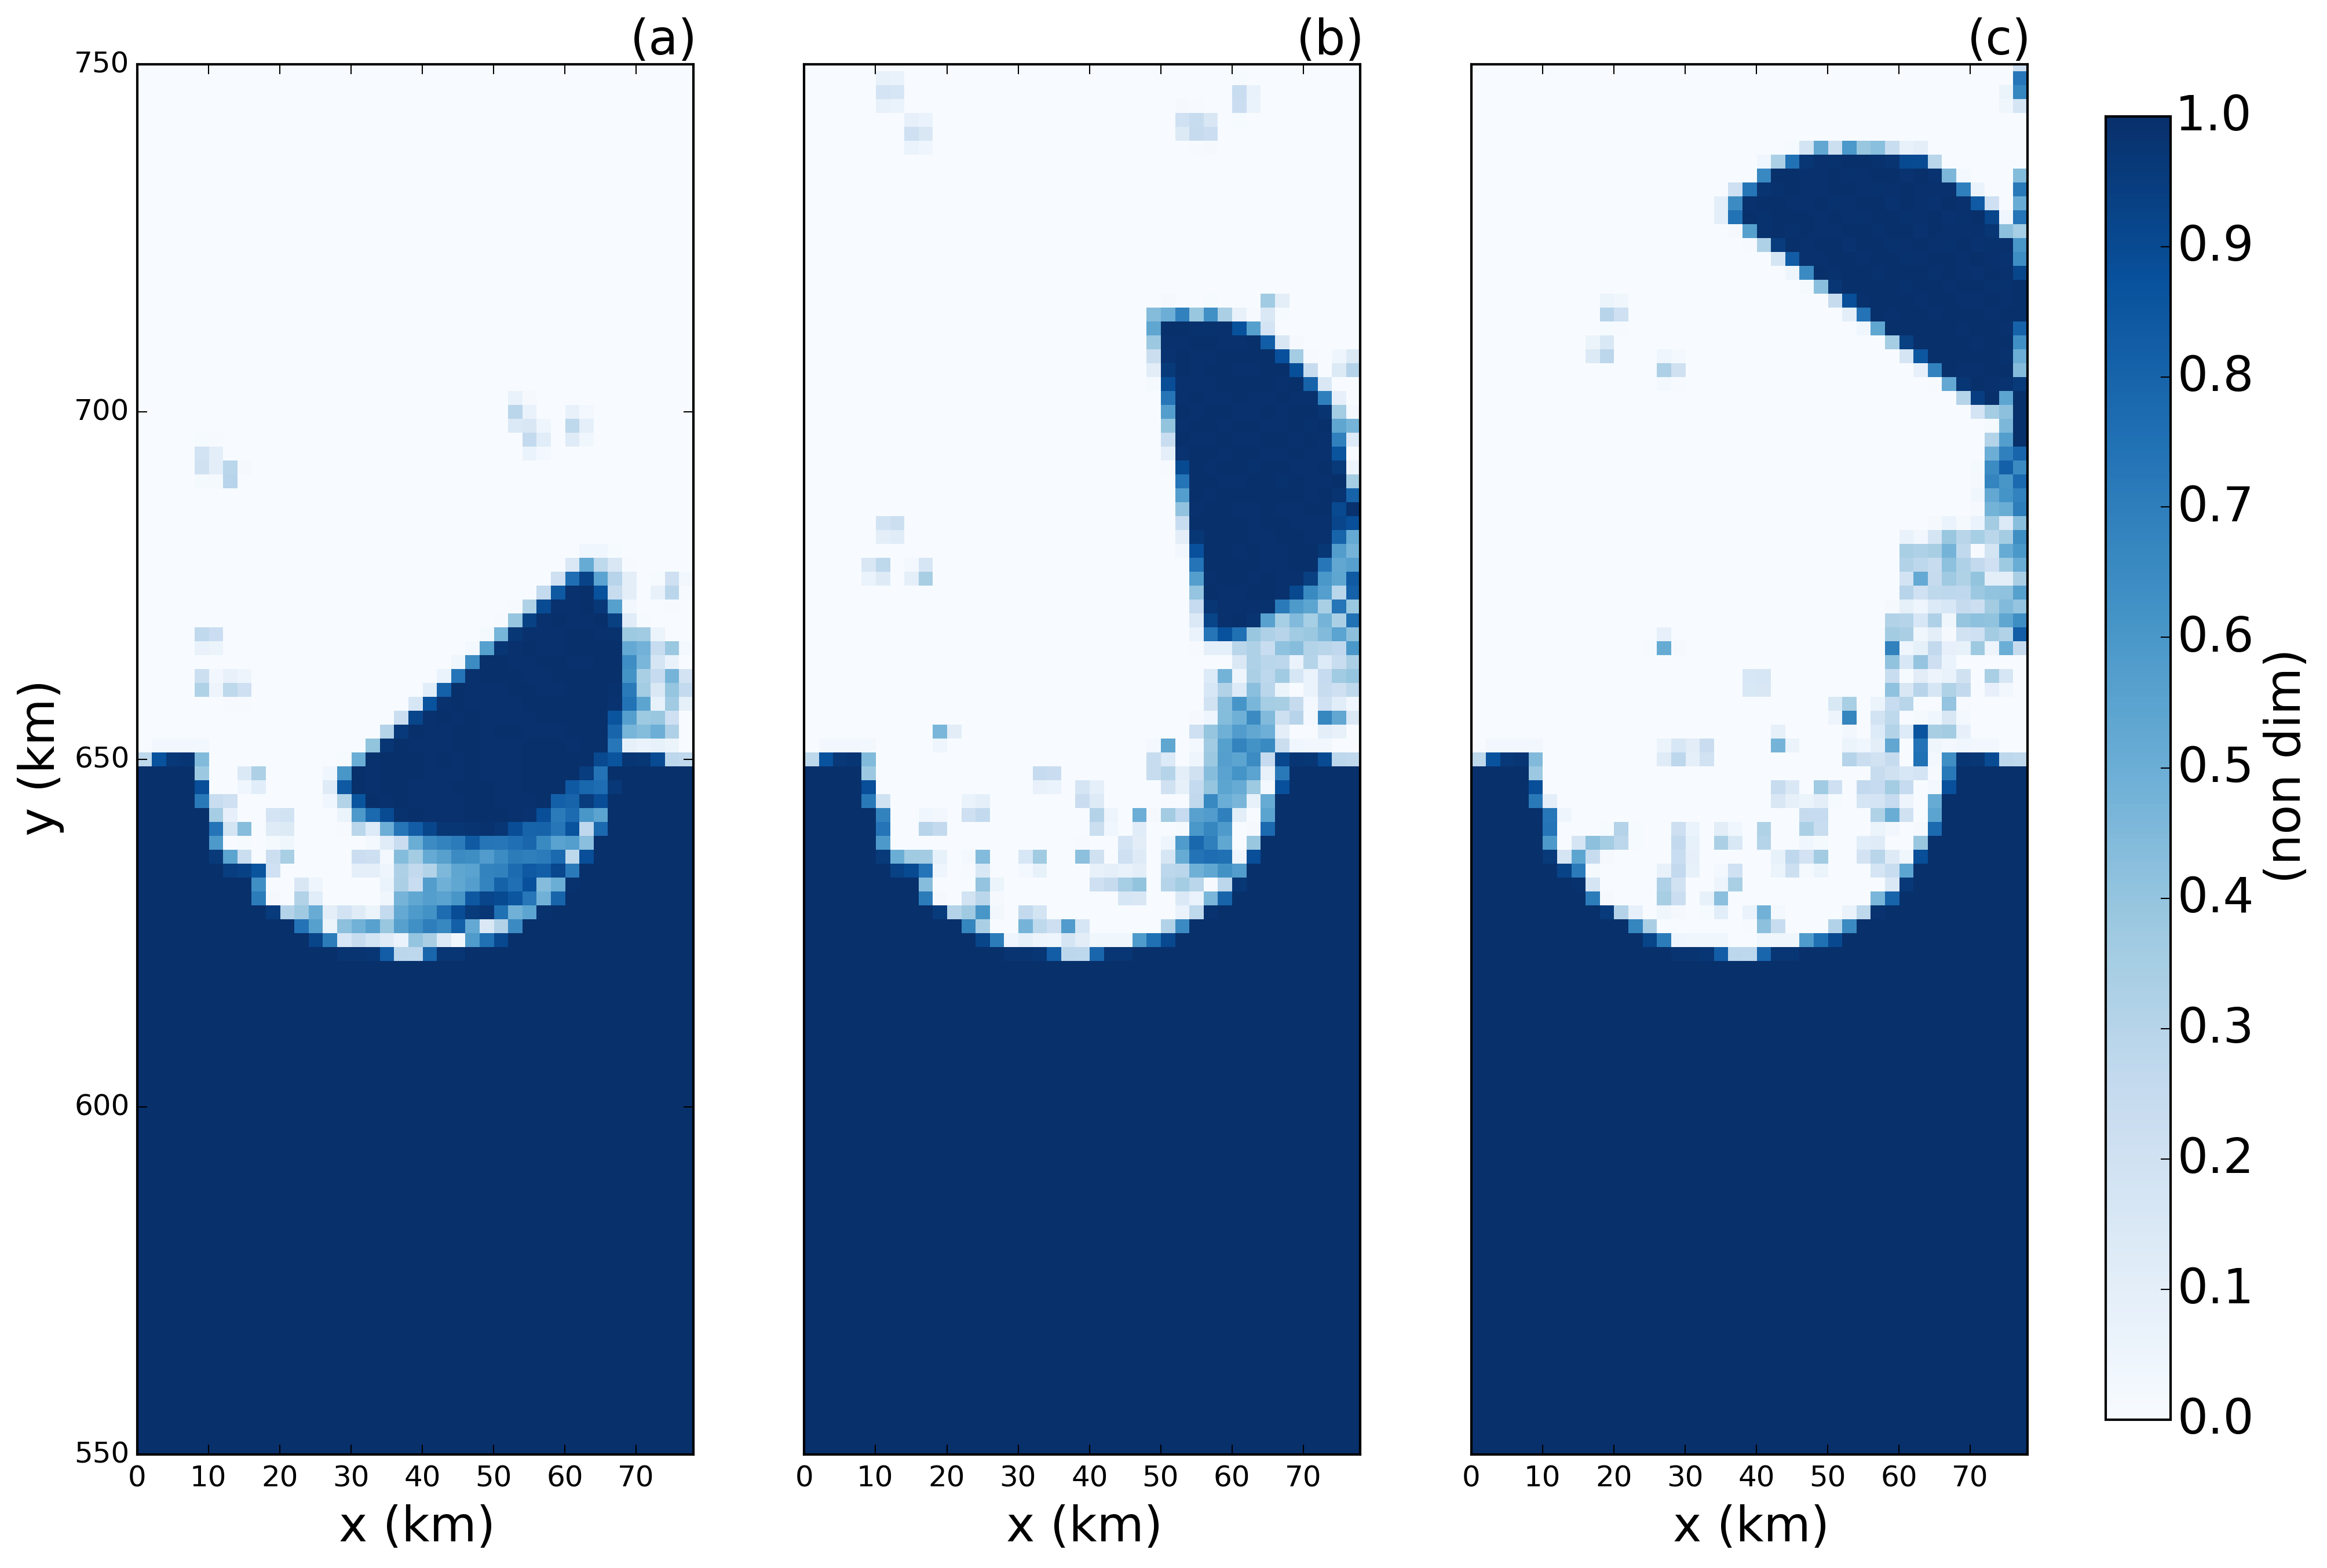
\includegraphics[width=0.99\textwidth]{/Users/alon/Desktop/files/Icebergs_clusters/Towards_Publication/Tech_paper/Github_stuff/Tech-paper/Figures/snapshots_ALE_z_Collapse_spread_area.png}
\caption{ {Snapshots of the fraction of ice cover in the LBIM tabular iceberg calving simulation. Snapshots are taken (a) 7, (b) 15, and (c) 30 days after calving. The dashed line in panel (c) shows the location of the vertical transects shown in Figure \ref{fig:Temperature_section_Collapse}}.}
\end{center}
\label{fig:Spread_area}
\end{figure}
 \clearpage


 

\begin{figure}
\begin{center}
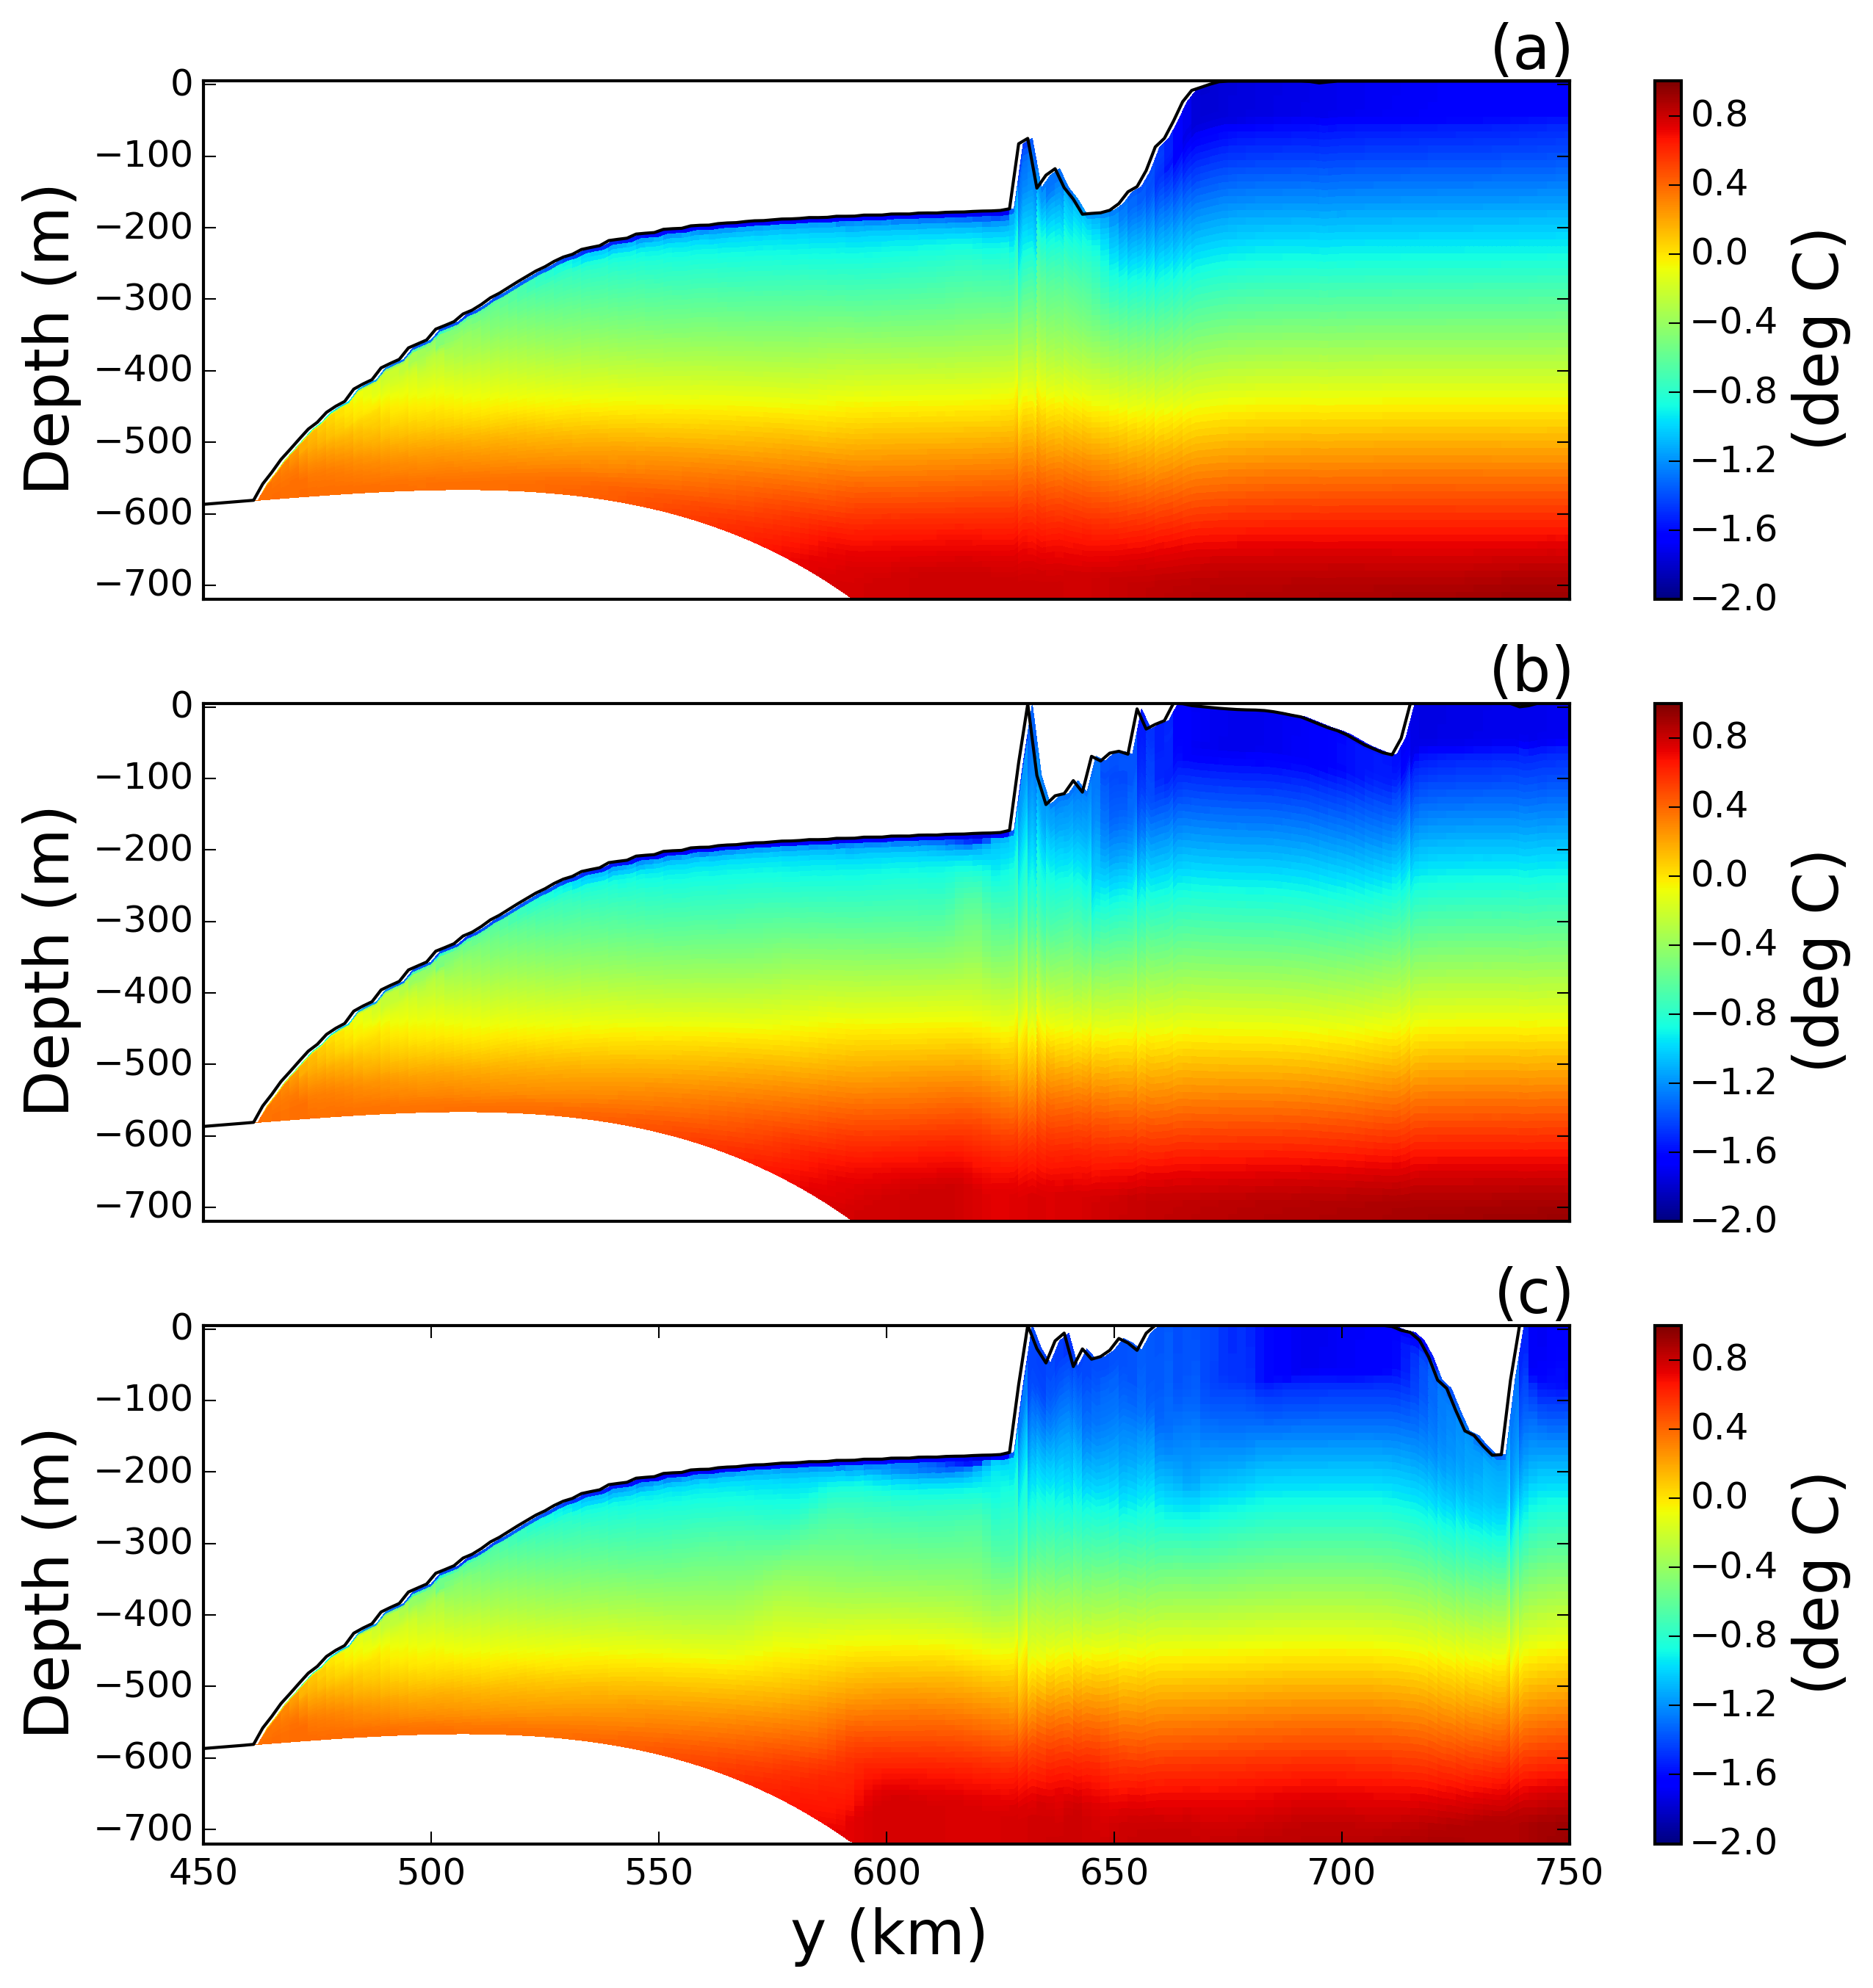
\includegraphics[width=0.99\textwidth]{/Users/alon/Desktop/files/Icebergs_clusters/Towards_Publication/Tech_paper/Github_stuff/Tech-paper/Figures/snapshots_ALE_z_Collapse_temp_layers_x10.png}
\caption{ {Snapshots of vertical sections of ocean temperature at $x=58 $km in the LBIM tabular iceberg calving experiment. Snapshots are taken (a) 7, (b) 15, and (c) 30 days after calving. The position of the vertical transects is shown by the dashed lines in Figure \ref{fig:Spread_area}c.}}
\end{center}
\label{fig:Temperature_section_Collapse}
\end{figure}
 \clearpage
 



\begin{figure}
\begin{center}
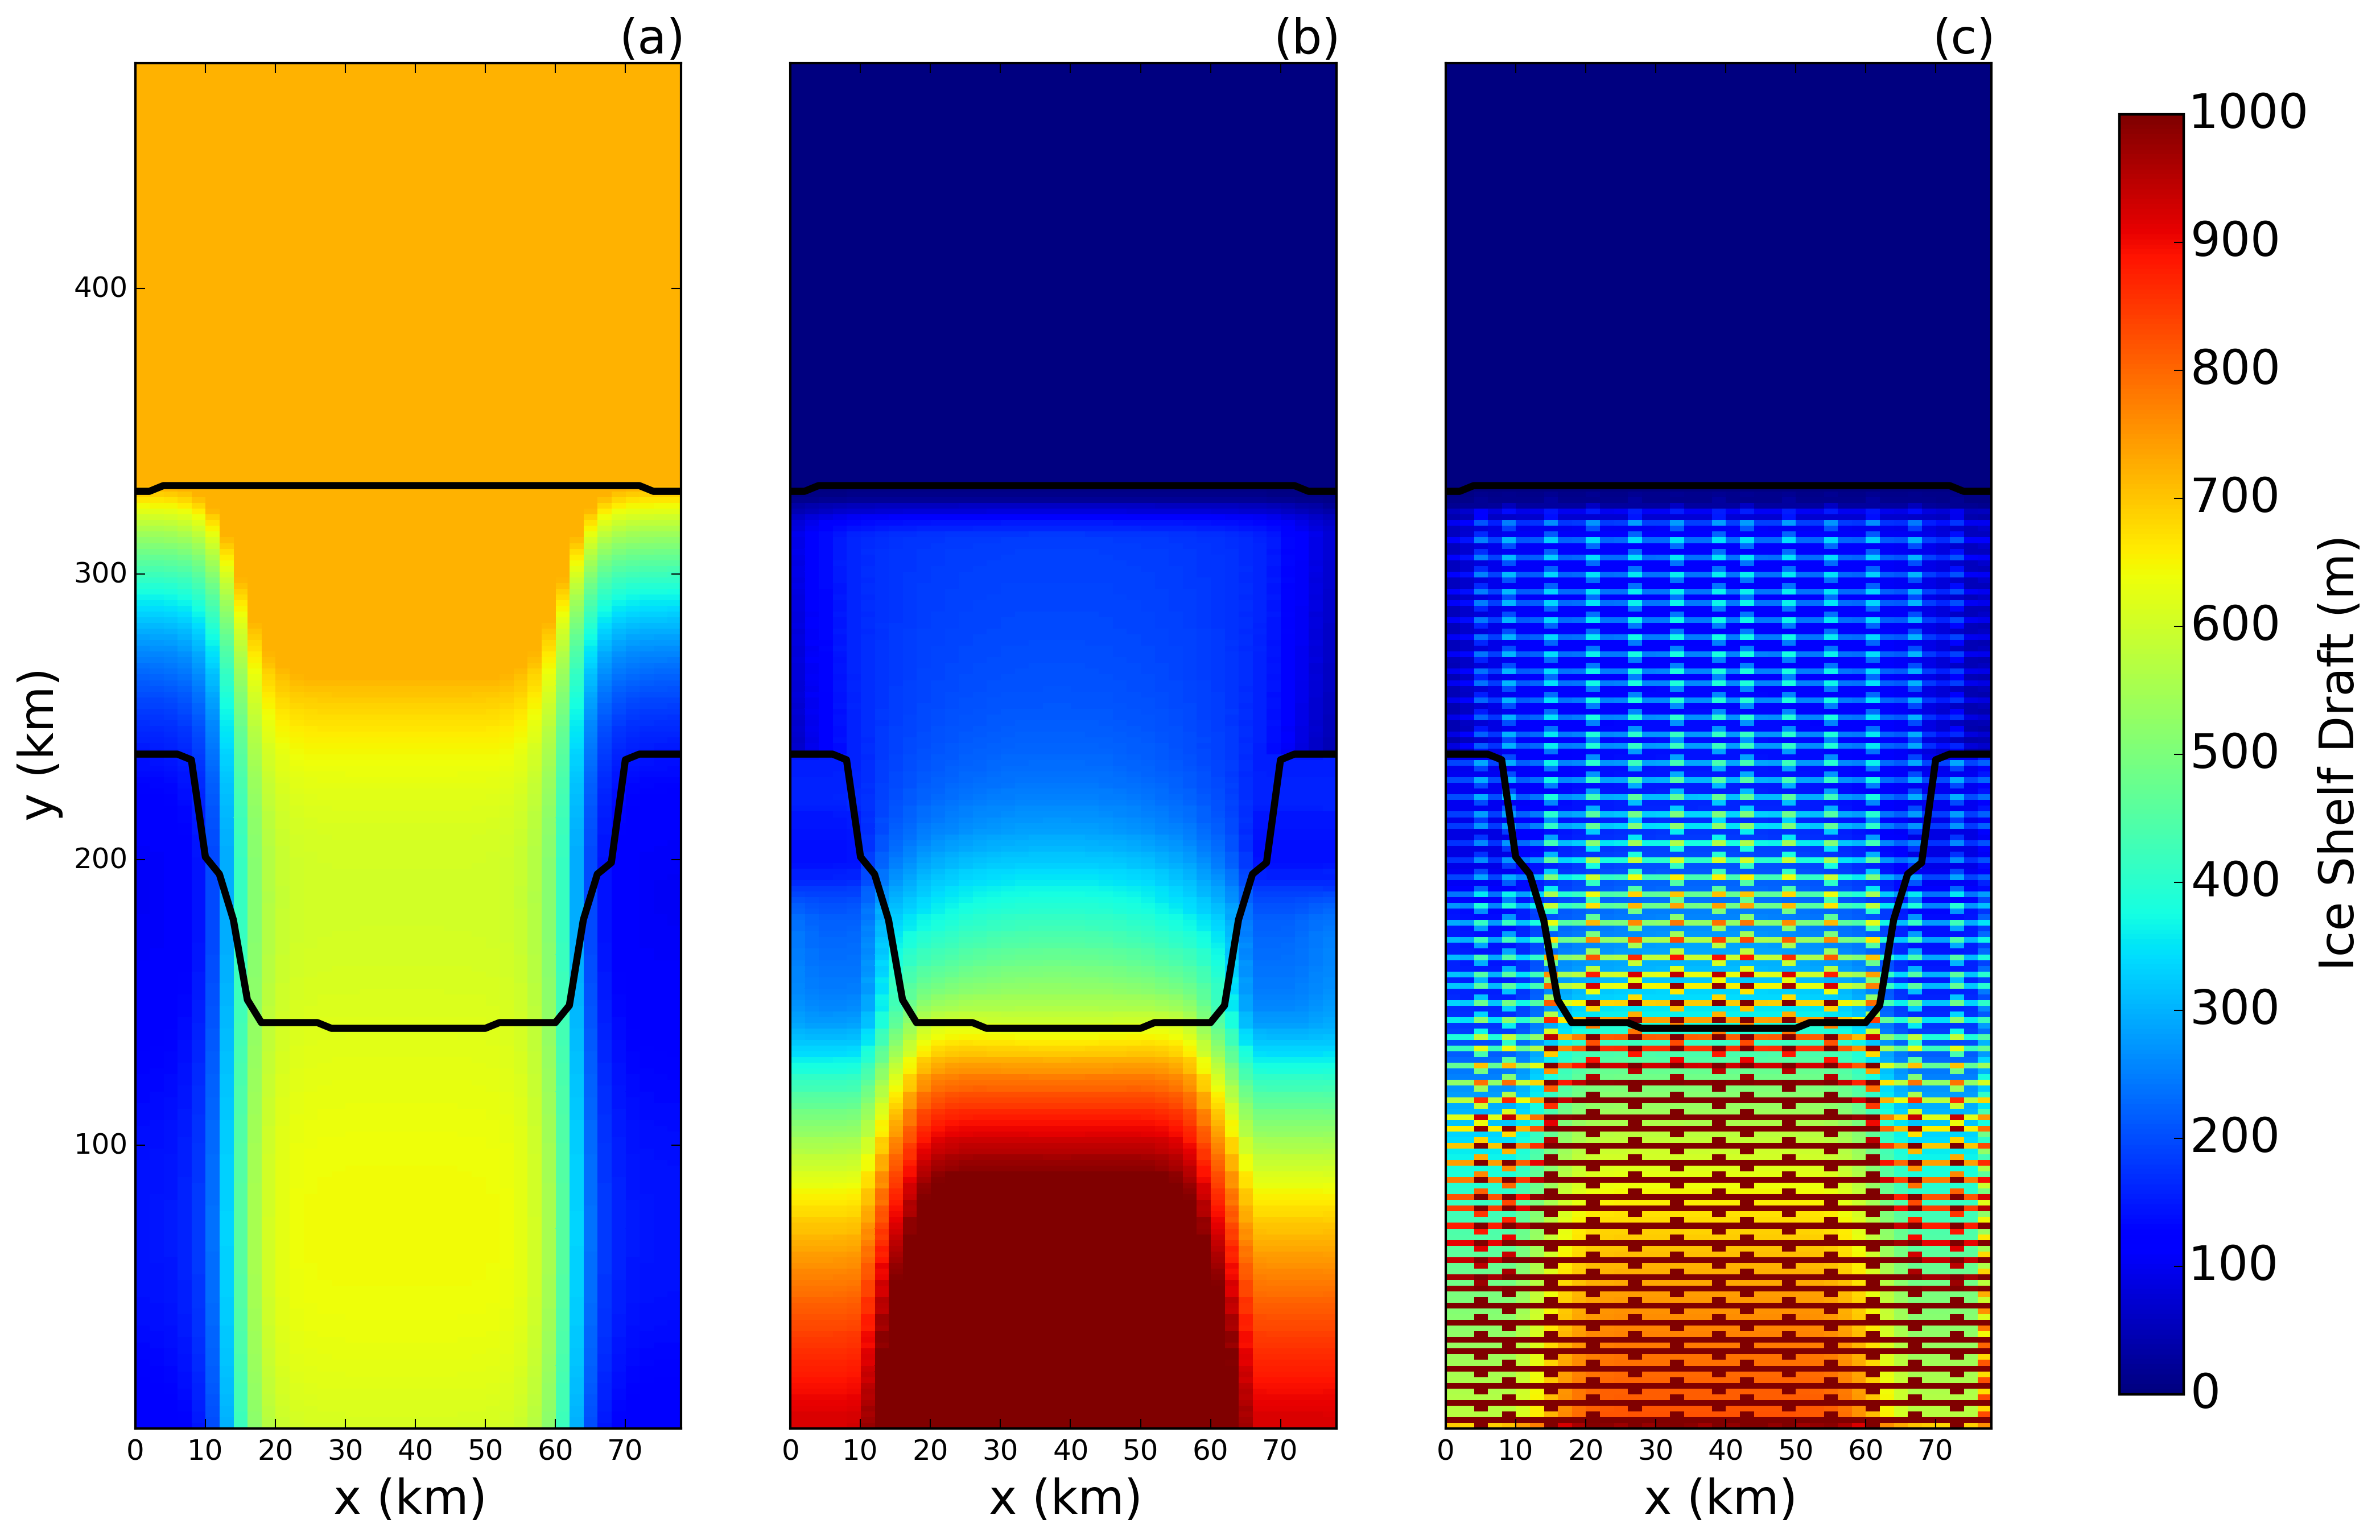
\includegraphics[width=0.99\textwidth]{/Users/alon/Desktop/files/Icebergs_clusters/Towards_Publication/Tech_paper/Github_stuff/Tech-paper/Figures/ALE_z_static_shelf_solo_D_spread_mass_mass.png}
\caption{ {(a) Ocean bottom topography and (b) ice-shelf draft used to initialized the tabular iceberg calving simulation. The ice draft is calculated from the total mass in an ocean grid cell after the mass-spreading interpolation has been applied (as explained in Section 2.2). (c) Initial ice draft that would be calculated if the mass-spreading interpolation were not used (i.e.: elements treated as point masses).}}
\end{center}
\label{fig:ISOMIP_mass_and_topog}
\end{figure}
 \clearpage
 
 


  
 \begin{figure}
\begin{center}
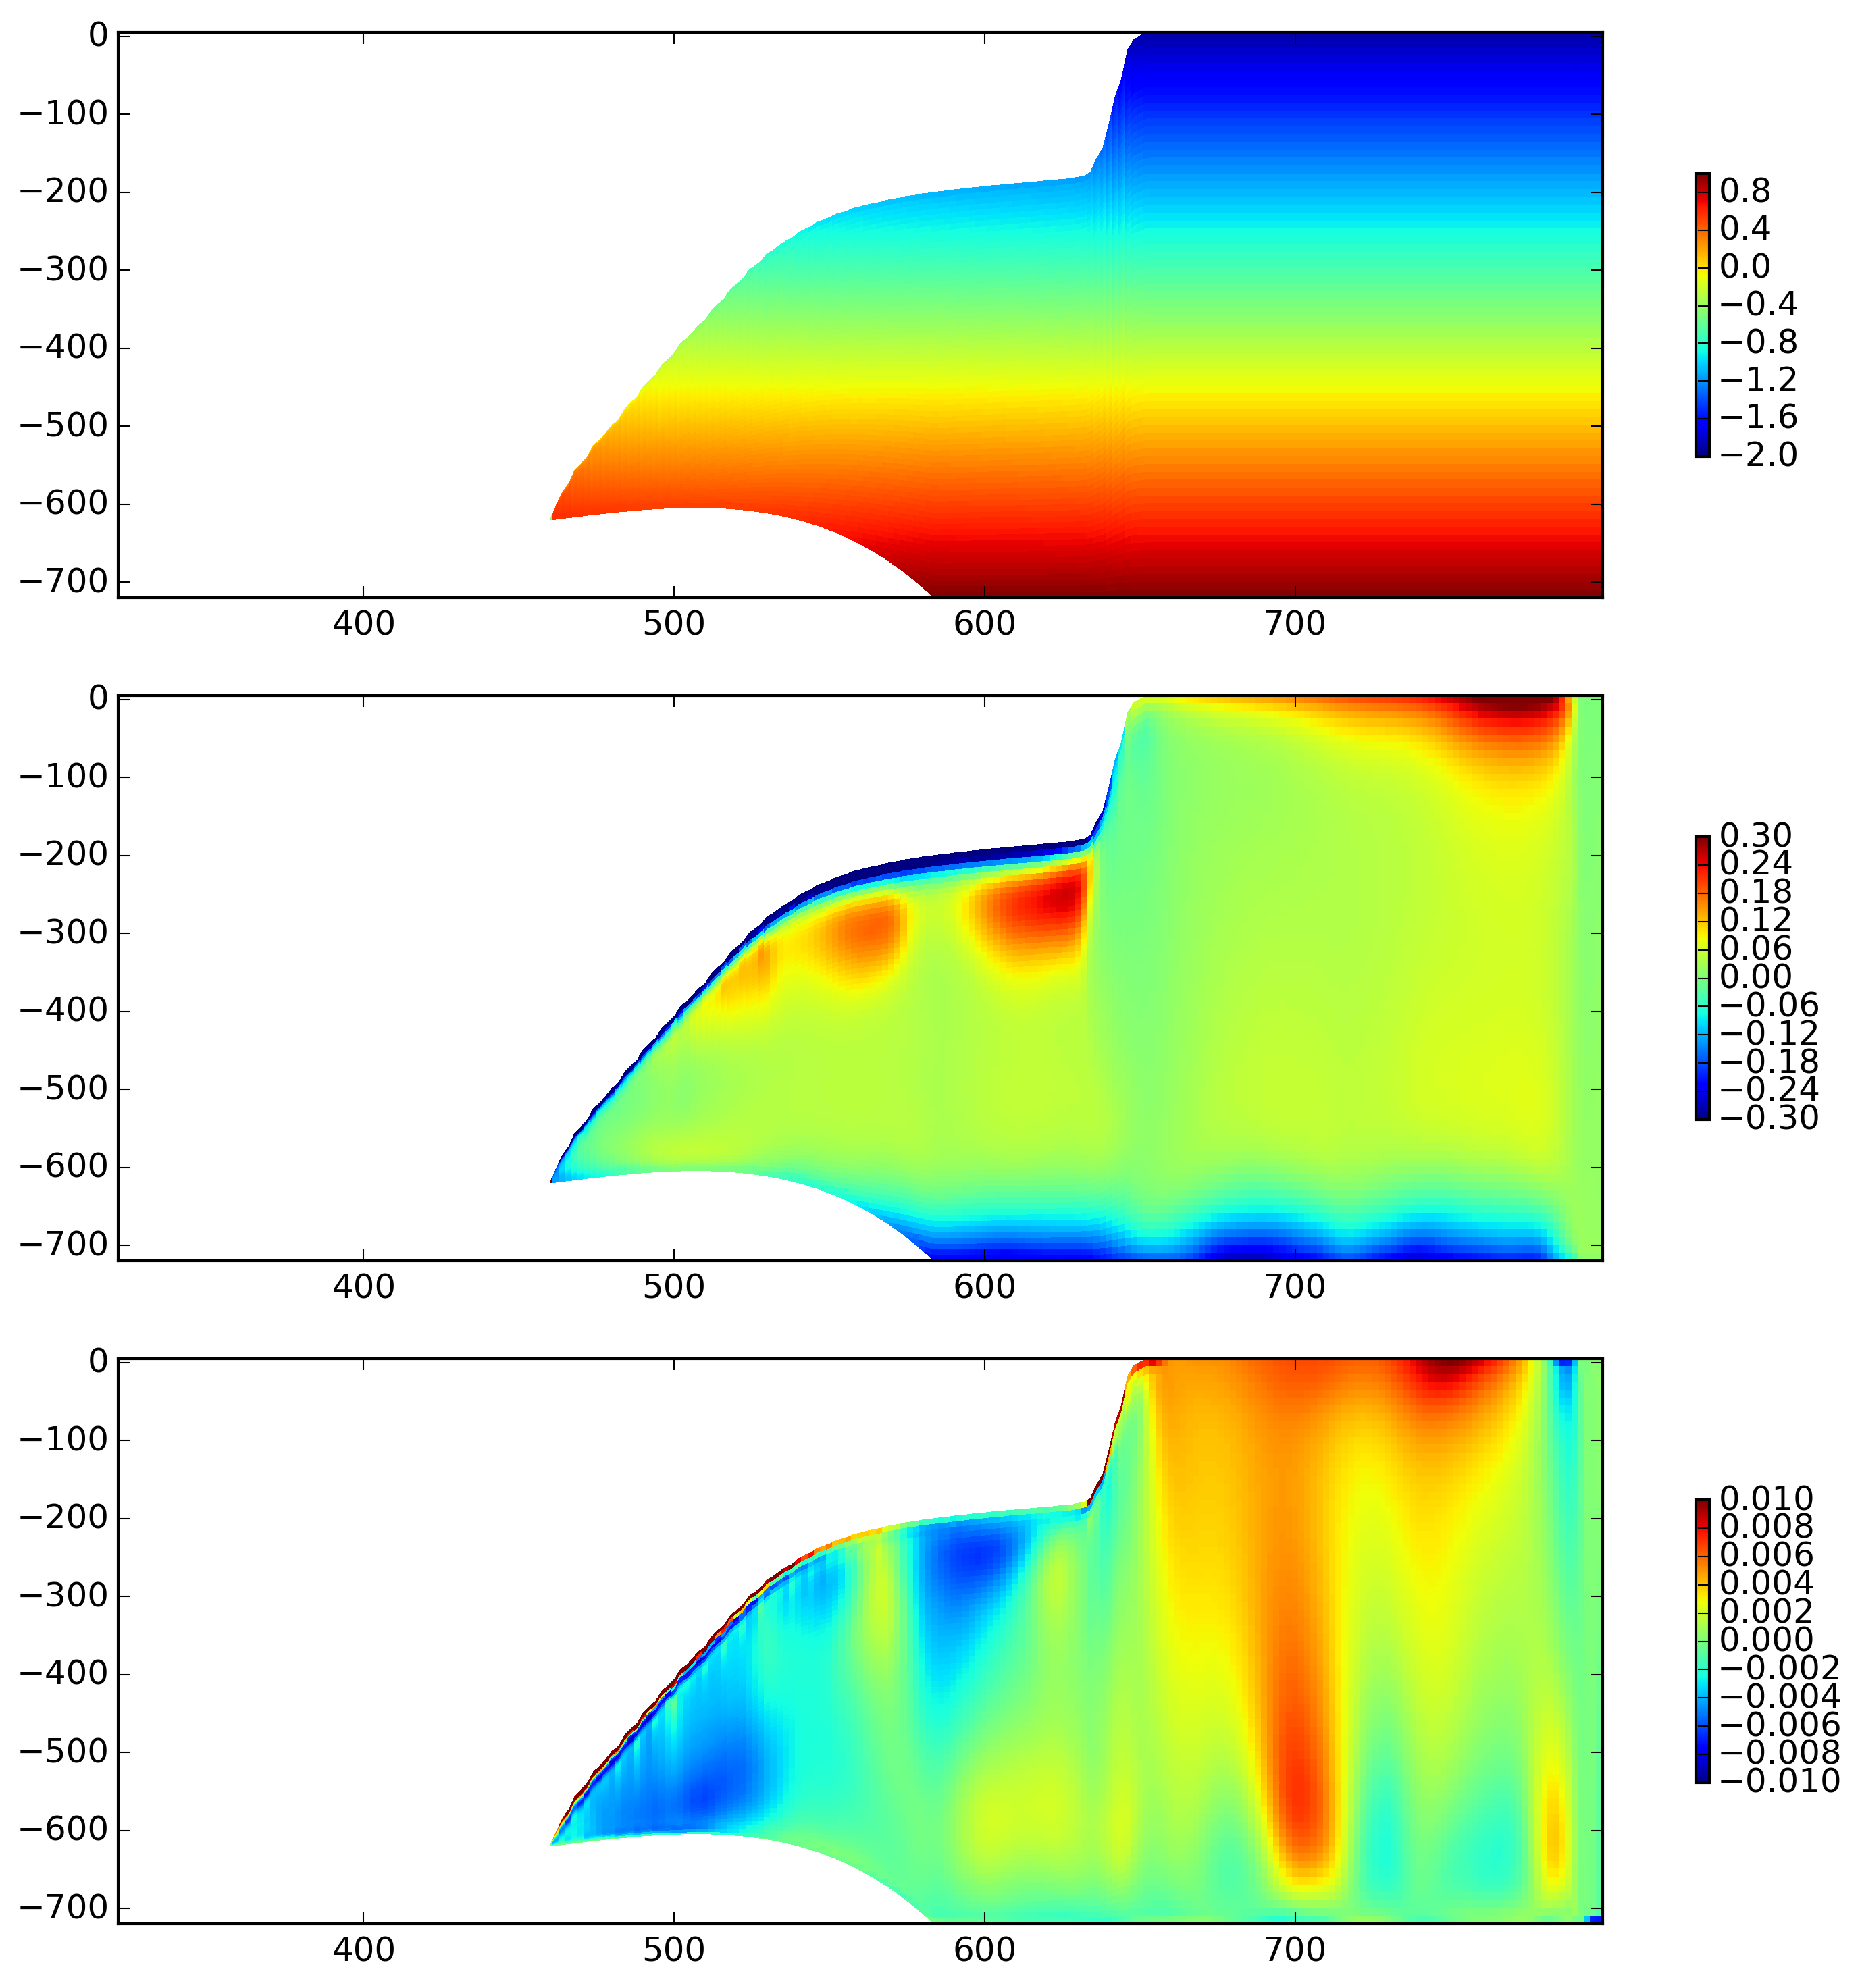
\includegraphics[width=0.99\textwidth]{/Users/alon/Desktop/files/Icebergs_clusters/Towards_Publication/Tech_paper/Github_stuff/Tech-paper/Figures/ALE_z_static_shelf_solo_temp_temp_v.png}
\caption{ {Results of the static ice-shelf experiment using the LIISM model coupled to MOM6. Panels show cross sections of the (a) initial temperature field, (b) temperature anomaly after 5-years (relative the the initial field), and (c) meridional velocity near the ice-shelf base after 5 years of simulation. The region shown in panel (c) is indicated by the black box on panel (b),}}
\end{center}
\label{fig:static_solo_temp_temp_v}
\end{figure} 
 \clearpage

 
\begin{figure}
\begin{center}
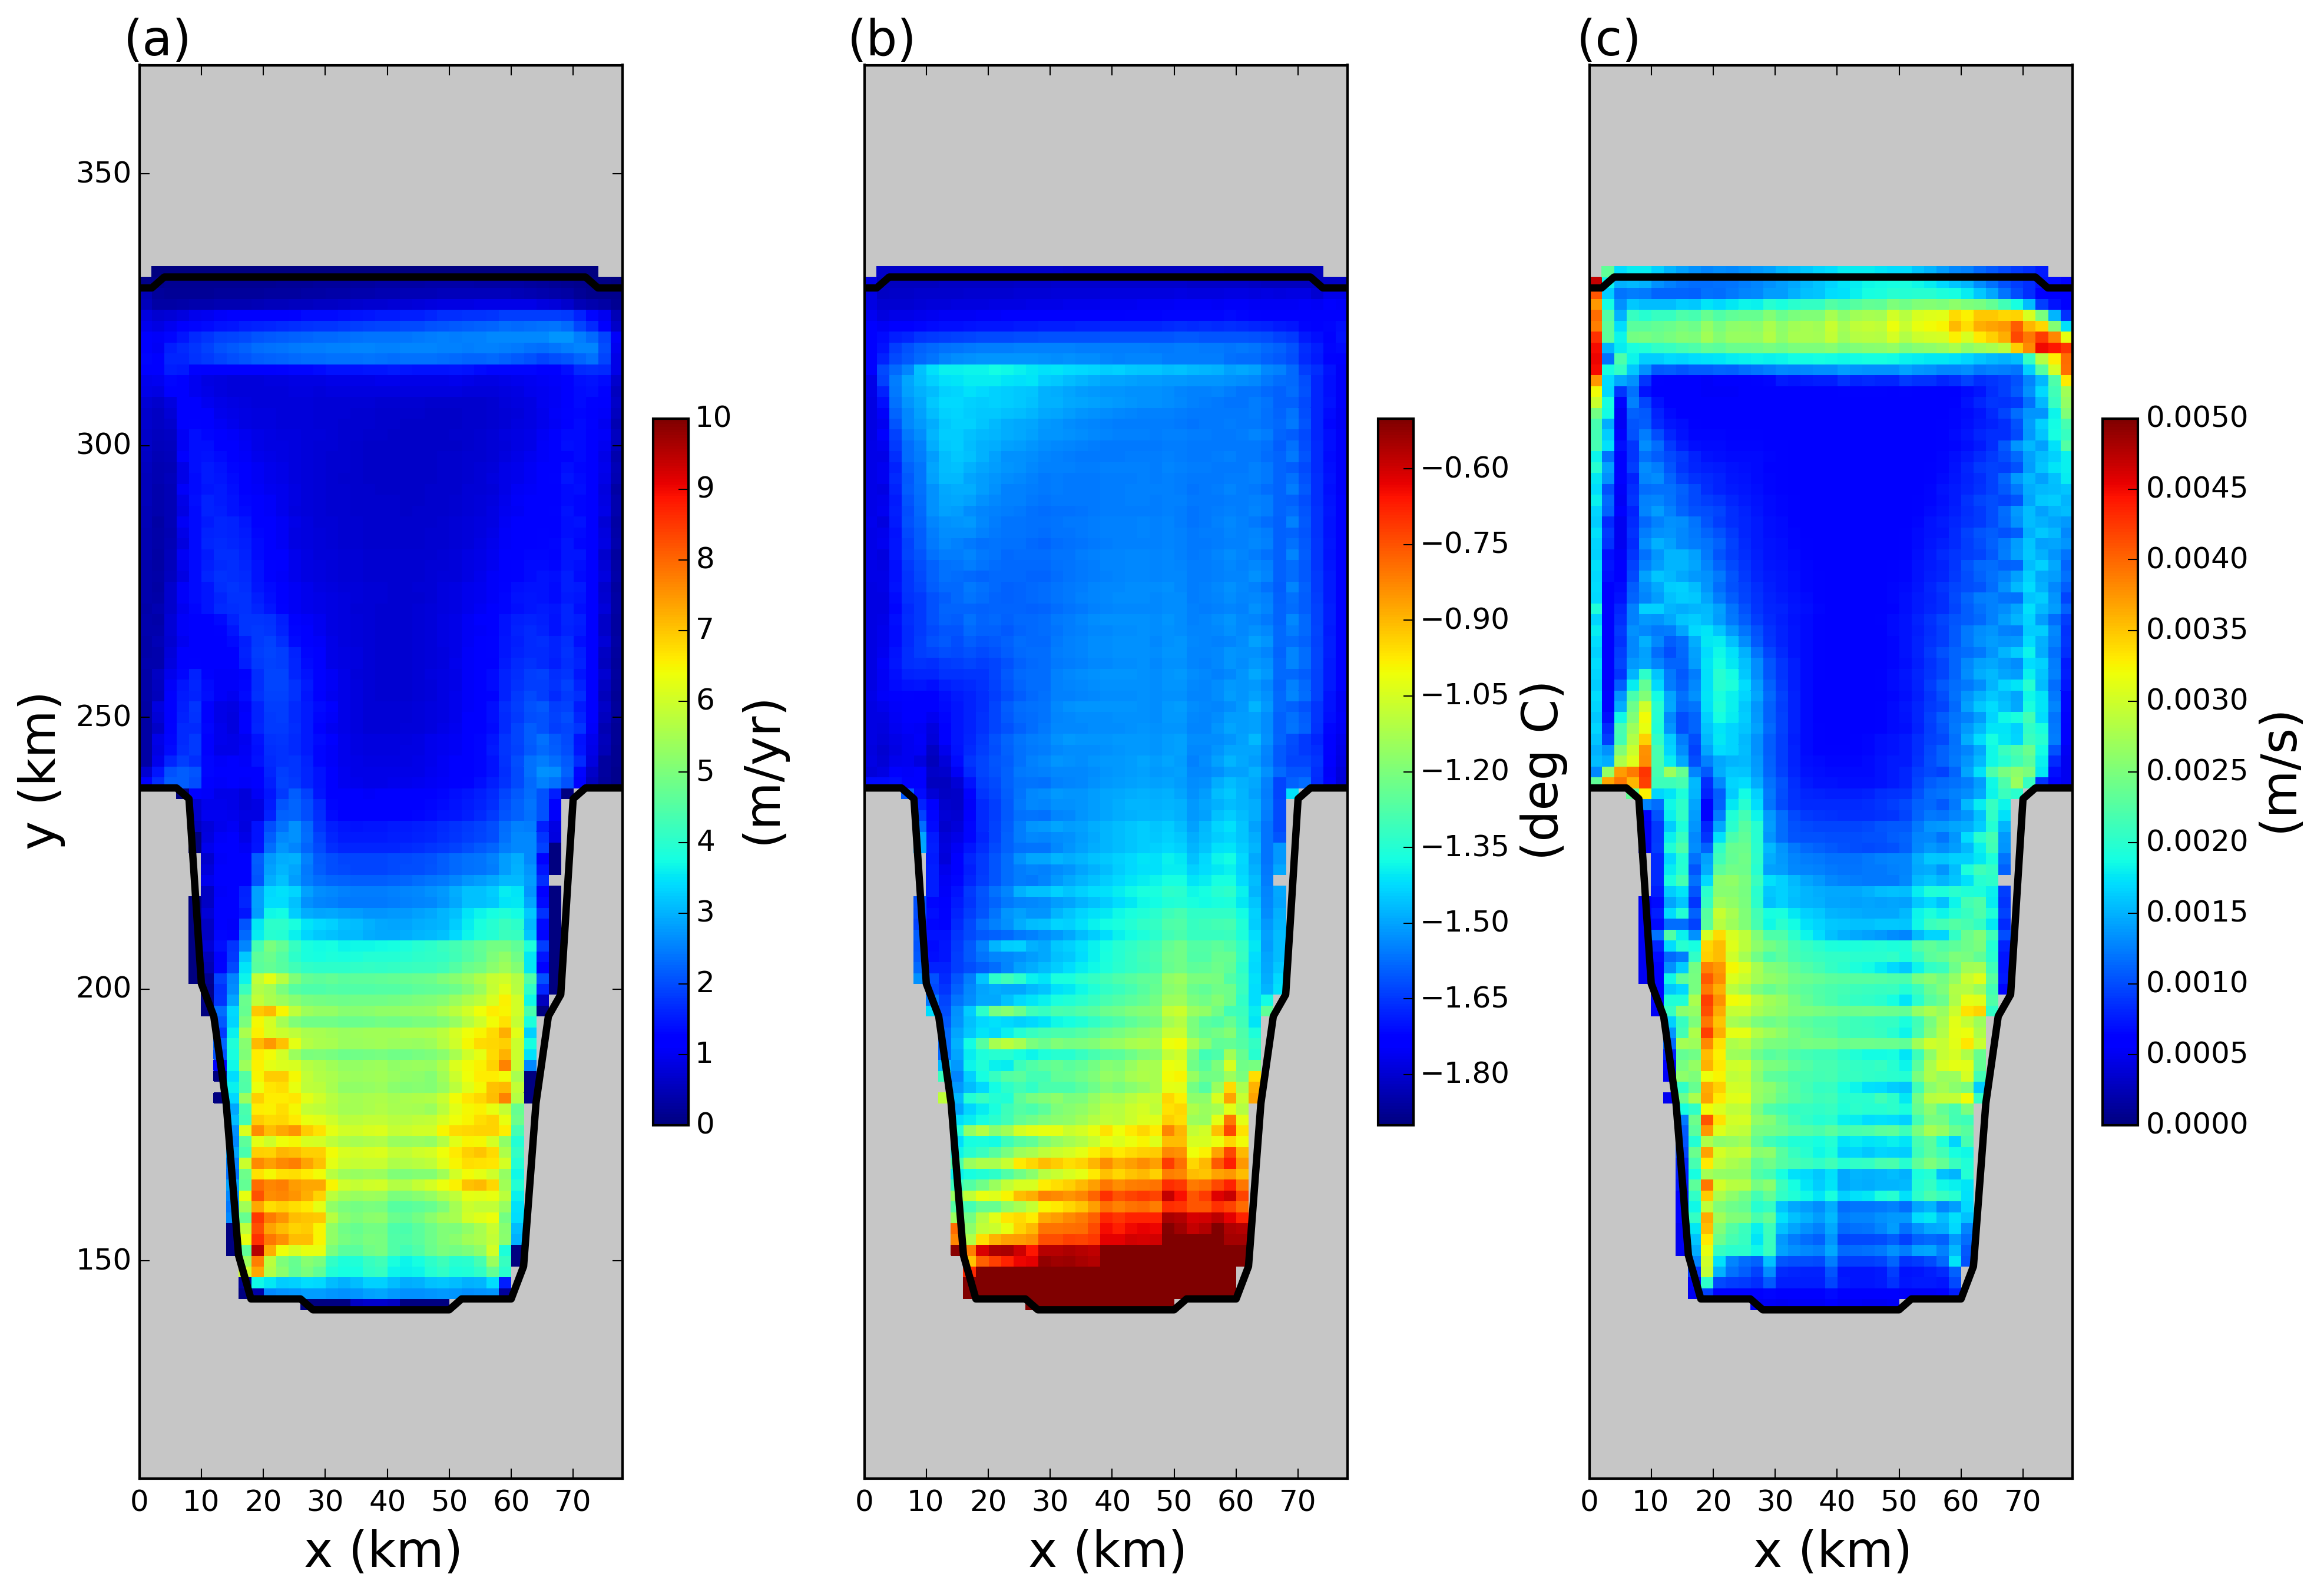
\includegraphics[width=0.99\textwidth]{/Users/alon/Desktop/files/Icebergs_clusters/Towards_Publication/Tech_paper/Github_stuff/Tech-paper/Figures/ALE_z_static_shelf_solo_melt_m_per_year_sst_ustar_iceberg.png}
\caption{ {Results of the static ice-shelf experiment using the LIISM model coupled to MOM6. The three panels show 5 year time average of the (a) melt rate, (b) top-of-ocean and (c) frictional velocity, $u^{*}$, at the base of the ice shelf. Fields are only shown in regions where the ice area fraction is $\geq 0.8$.}}
\end{center}
\label{fig:static_solo_melt}
\end{figure} 
 \clearpage



\begin{figure}
\begin{center}
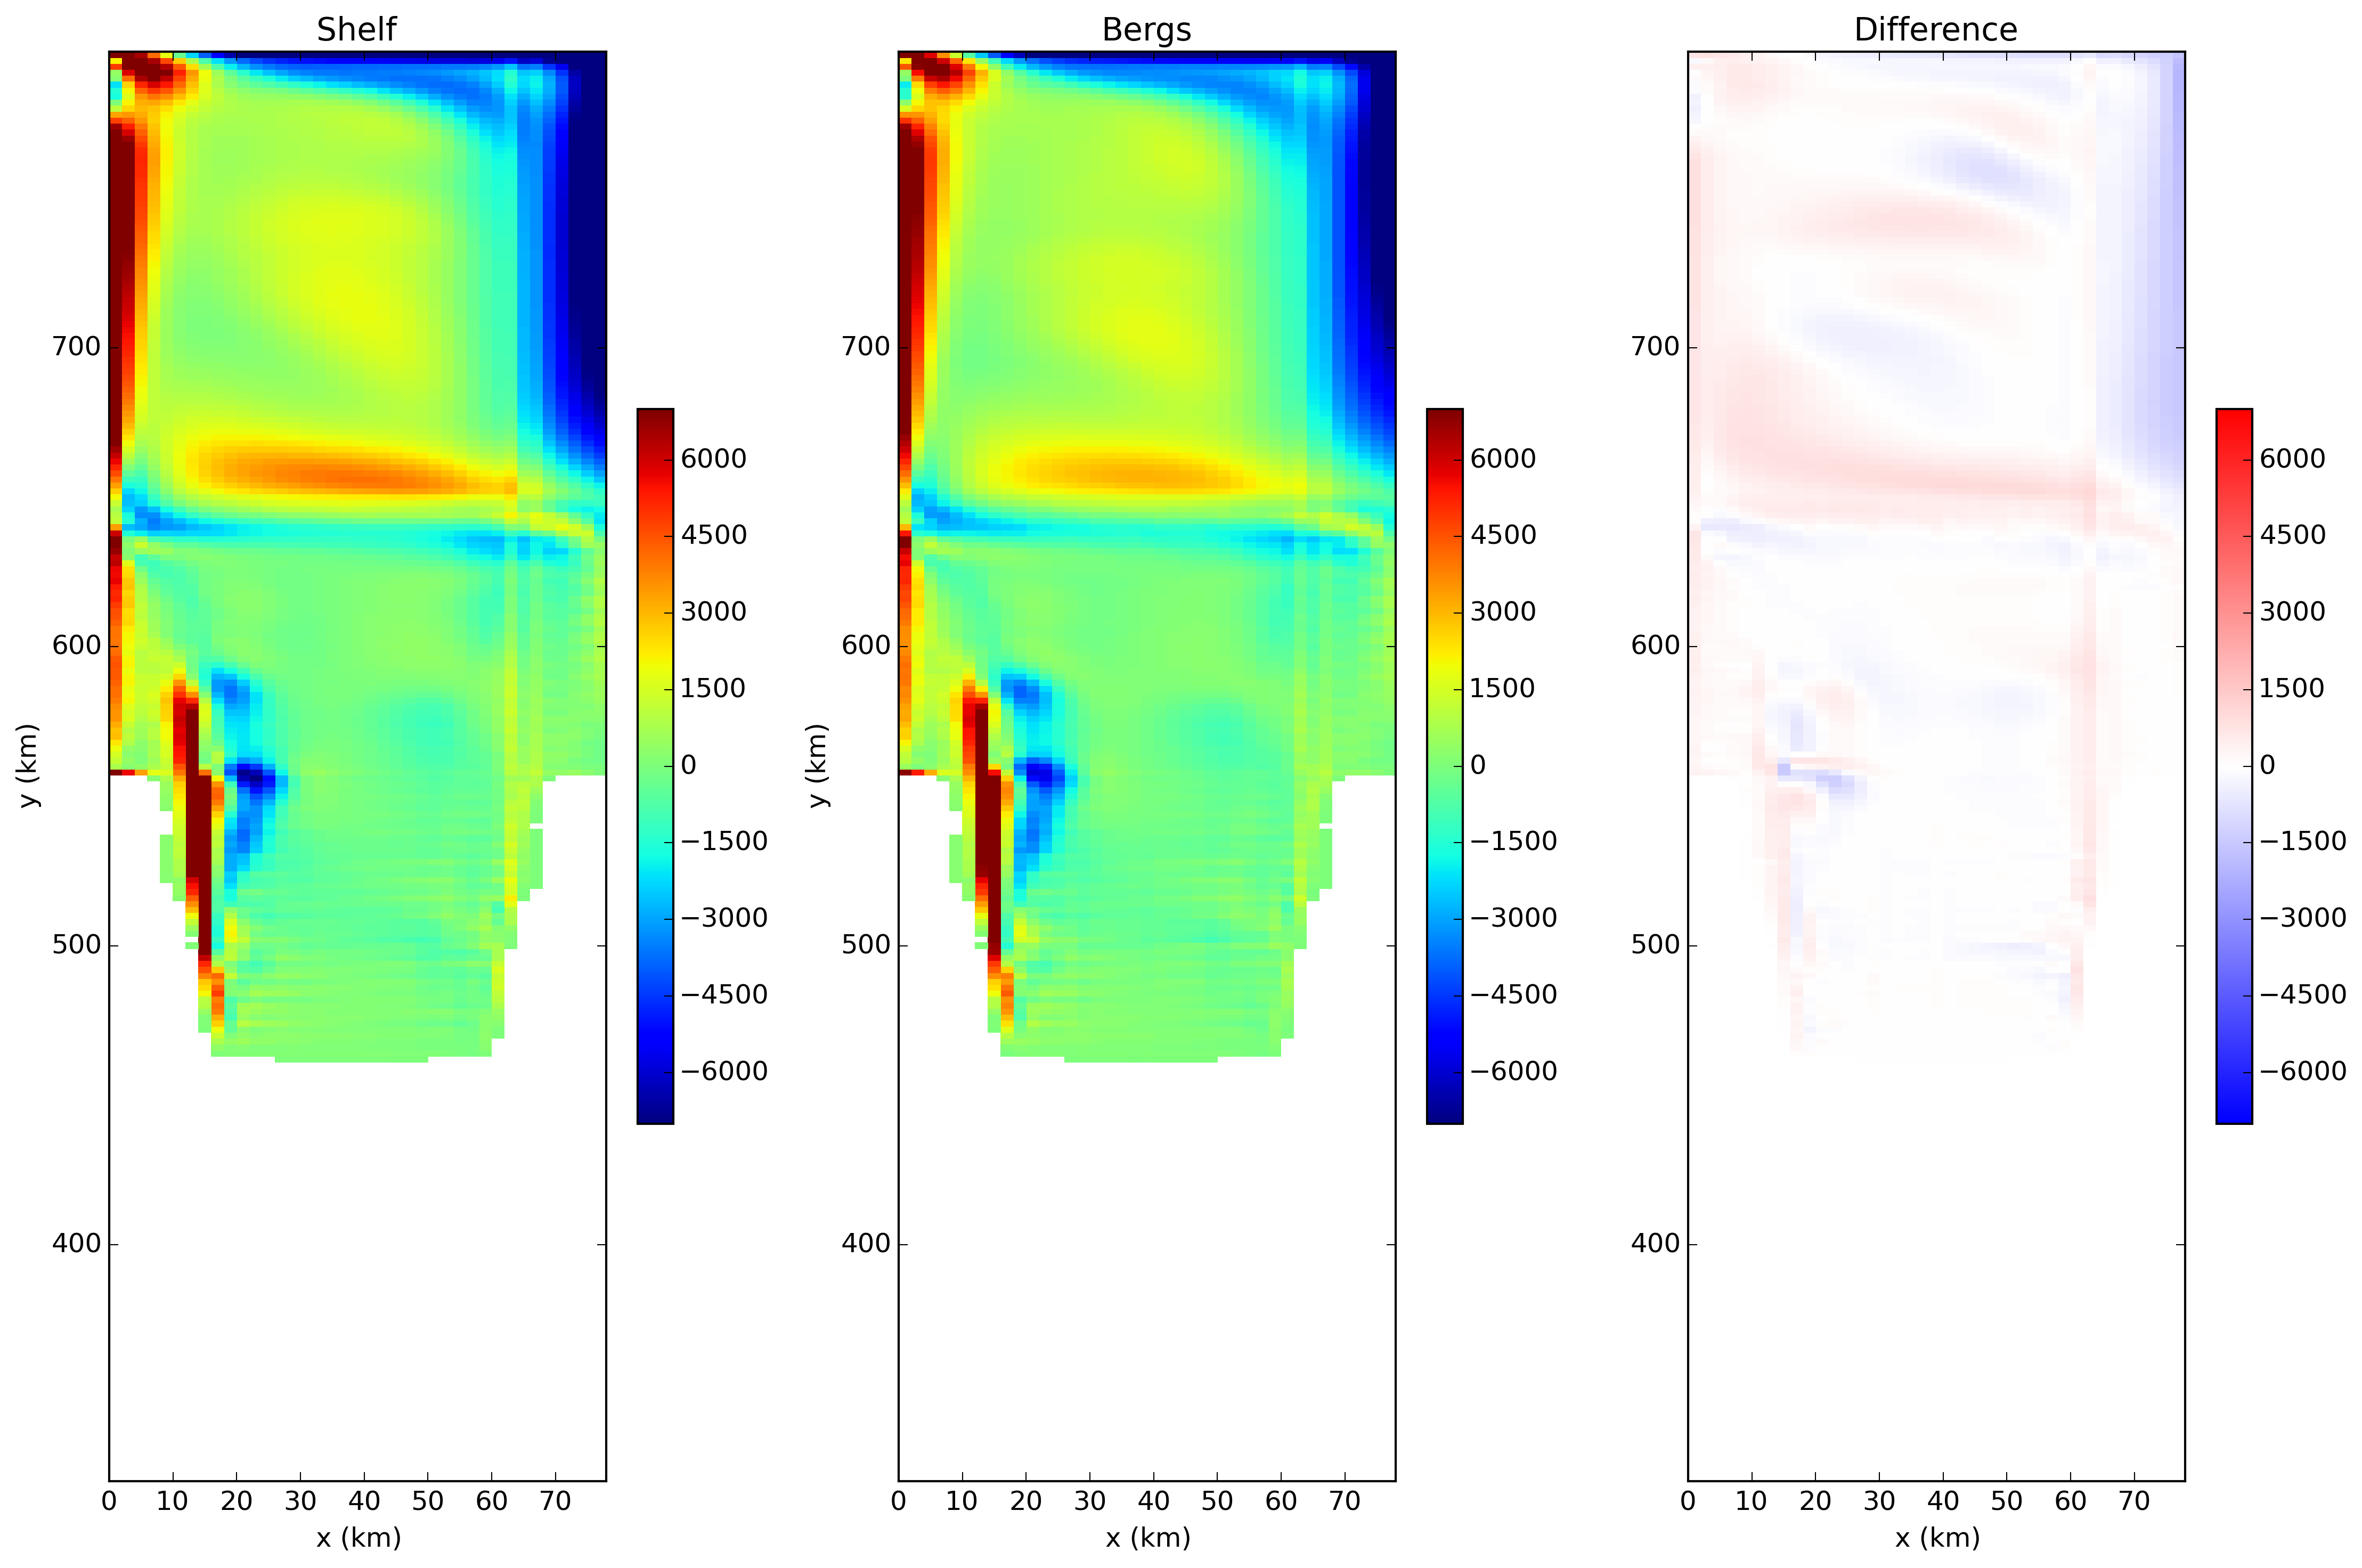
\includegraphics[width=0.99\textwidth]{/Users/alon/Desktop/files/Icebergs_clusters/Towards_Publication/Tech_paper/Github_stuff/Tech-paper/Figures/ALE_z_static_shelf_comparison_barotropic_sf.png}
\caption{ {Time-averaged barotropic stream function in the (a) Lagrangian and (b) Eularian simulations in the static ice-shelf configuration. Panel (c) shows the difference between panels (a) and (b). The time averages are taken over 5 years of model time, beginning at the end of the 5 year spin up period.}}
\end{center}
%FIgure created by \end{center}
\label{fig:Bt_comparison}
\end{figure}
 \clearpage



\begin{figure}
\begin{center}
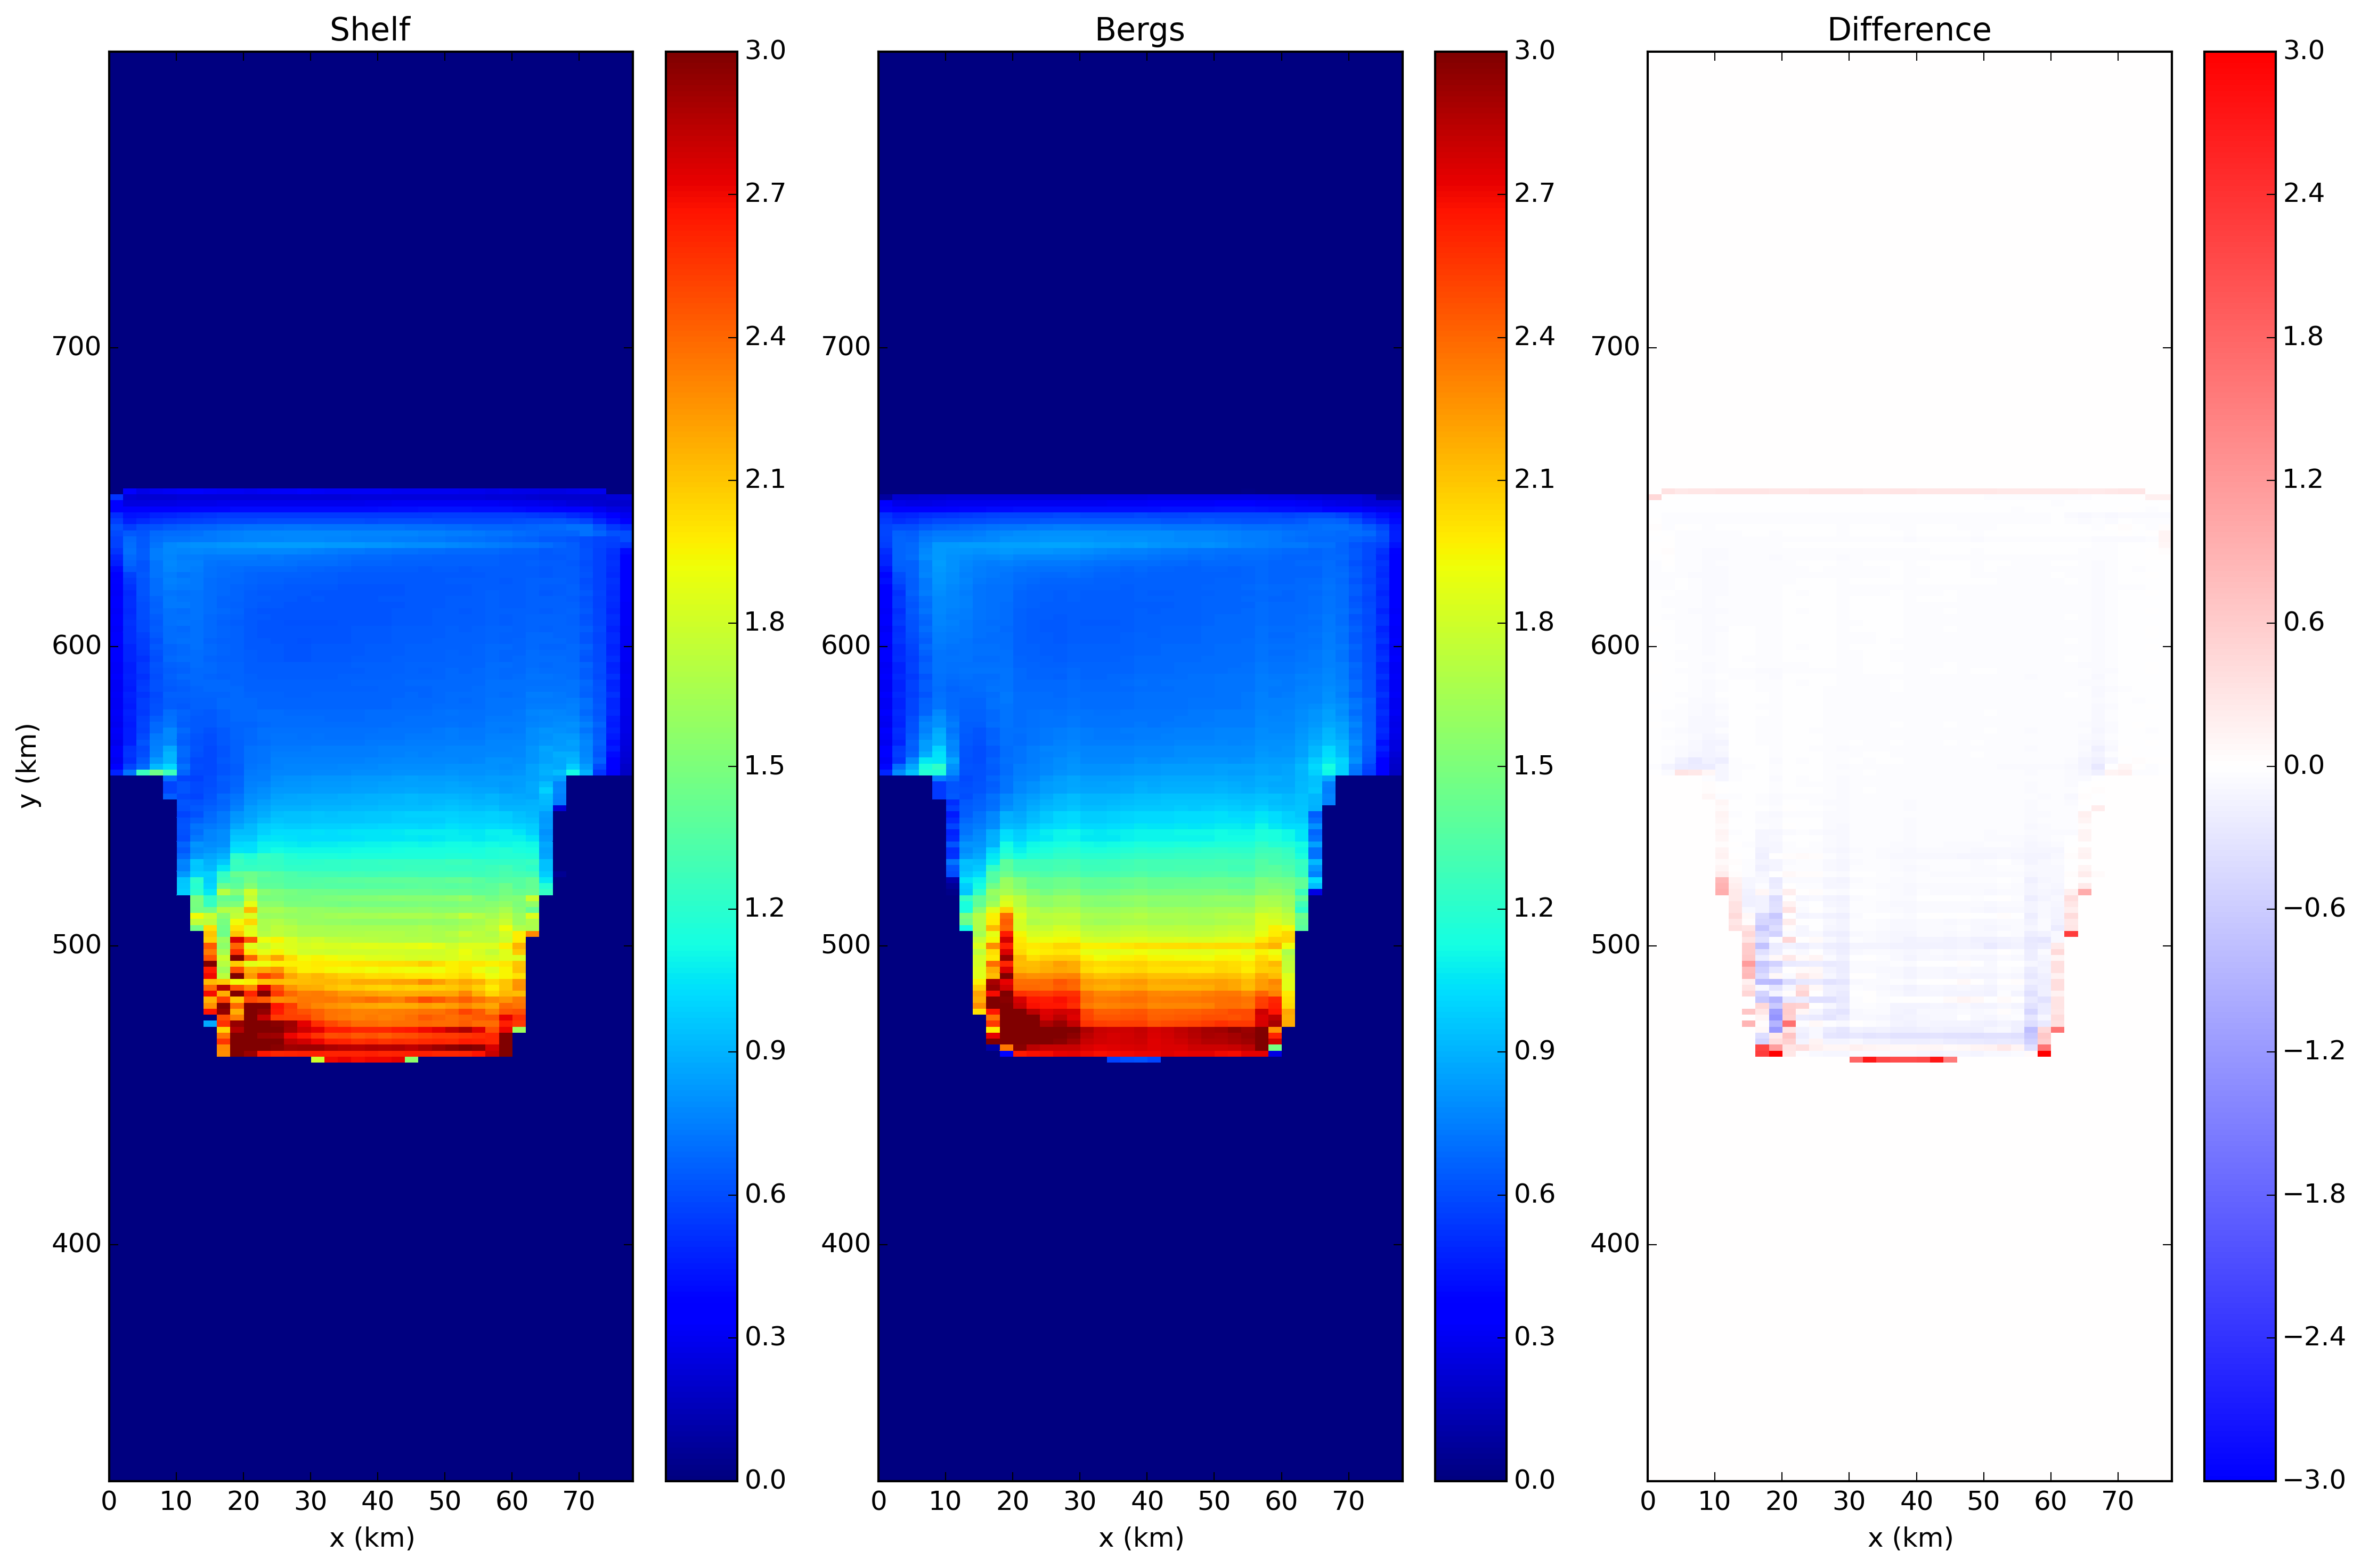
\includegraphics[width=0.99\textwidth]{/Users/alon/Desktop/files/Icebergs_clusters/Towards_Publication/Tech_paper/Github_stuff/Tech-paper/Figures/static_shelf_comparison_melt.png}
\caption{ {Comparison of Eulerian ice-shelf model and Lagrangian Ice shelf model melt fields.}}
\end{center}
\label{fig:Melt_comparison}
\end{figure}
 \clearpage


\begin{figure}
\begin{center}
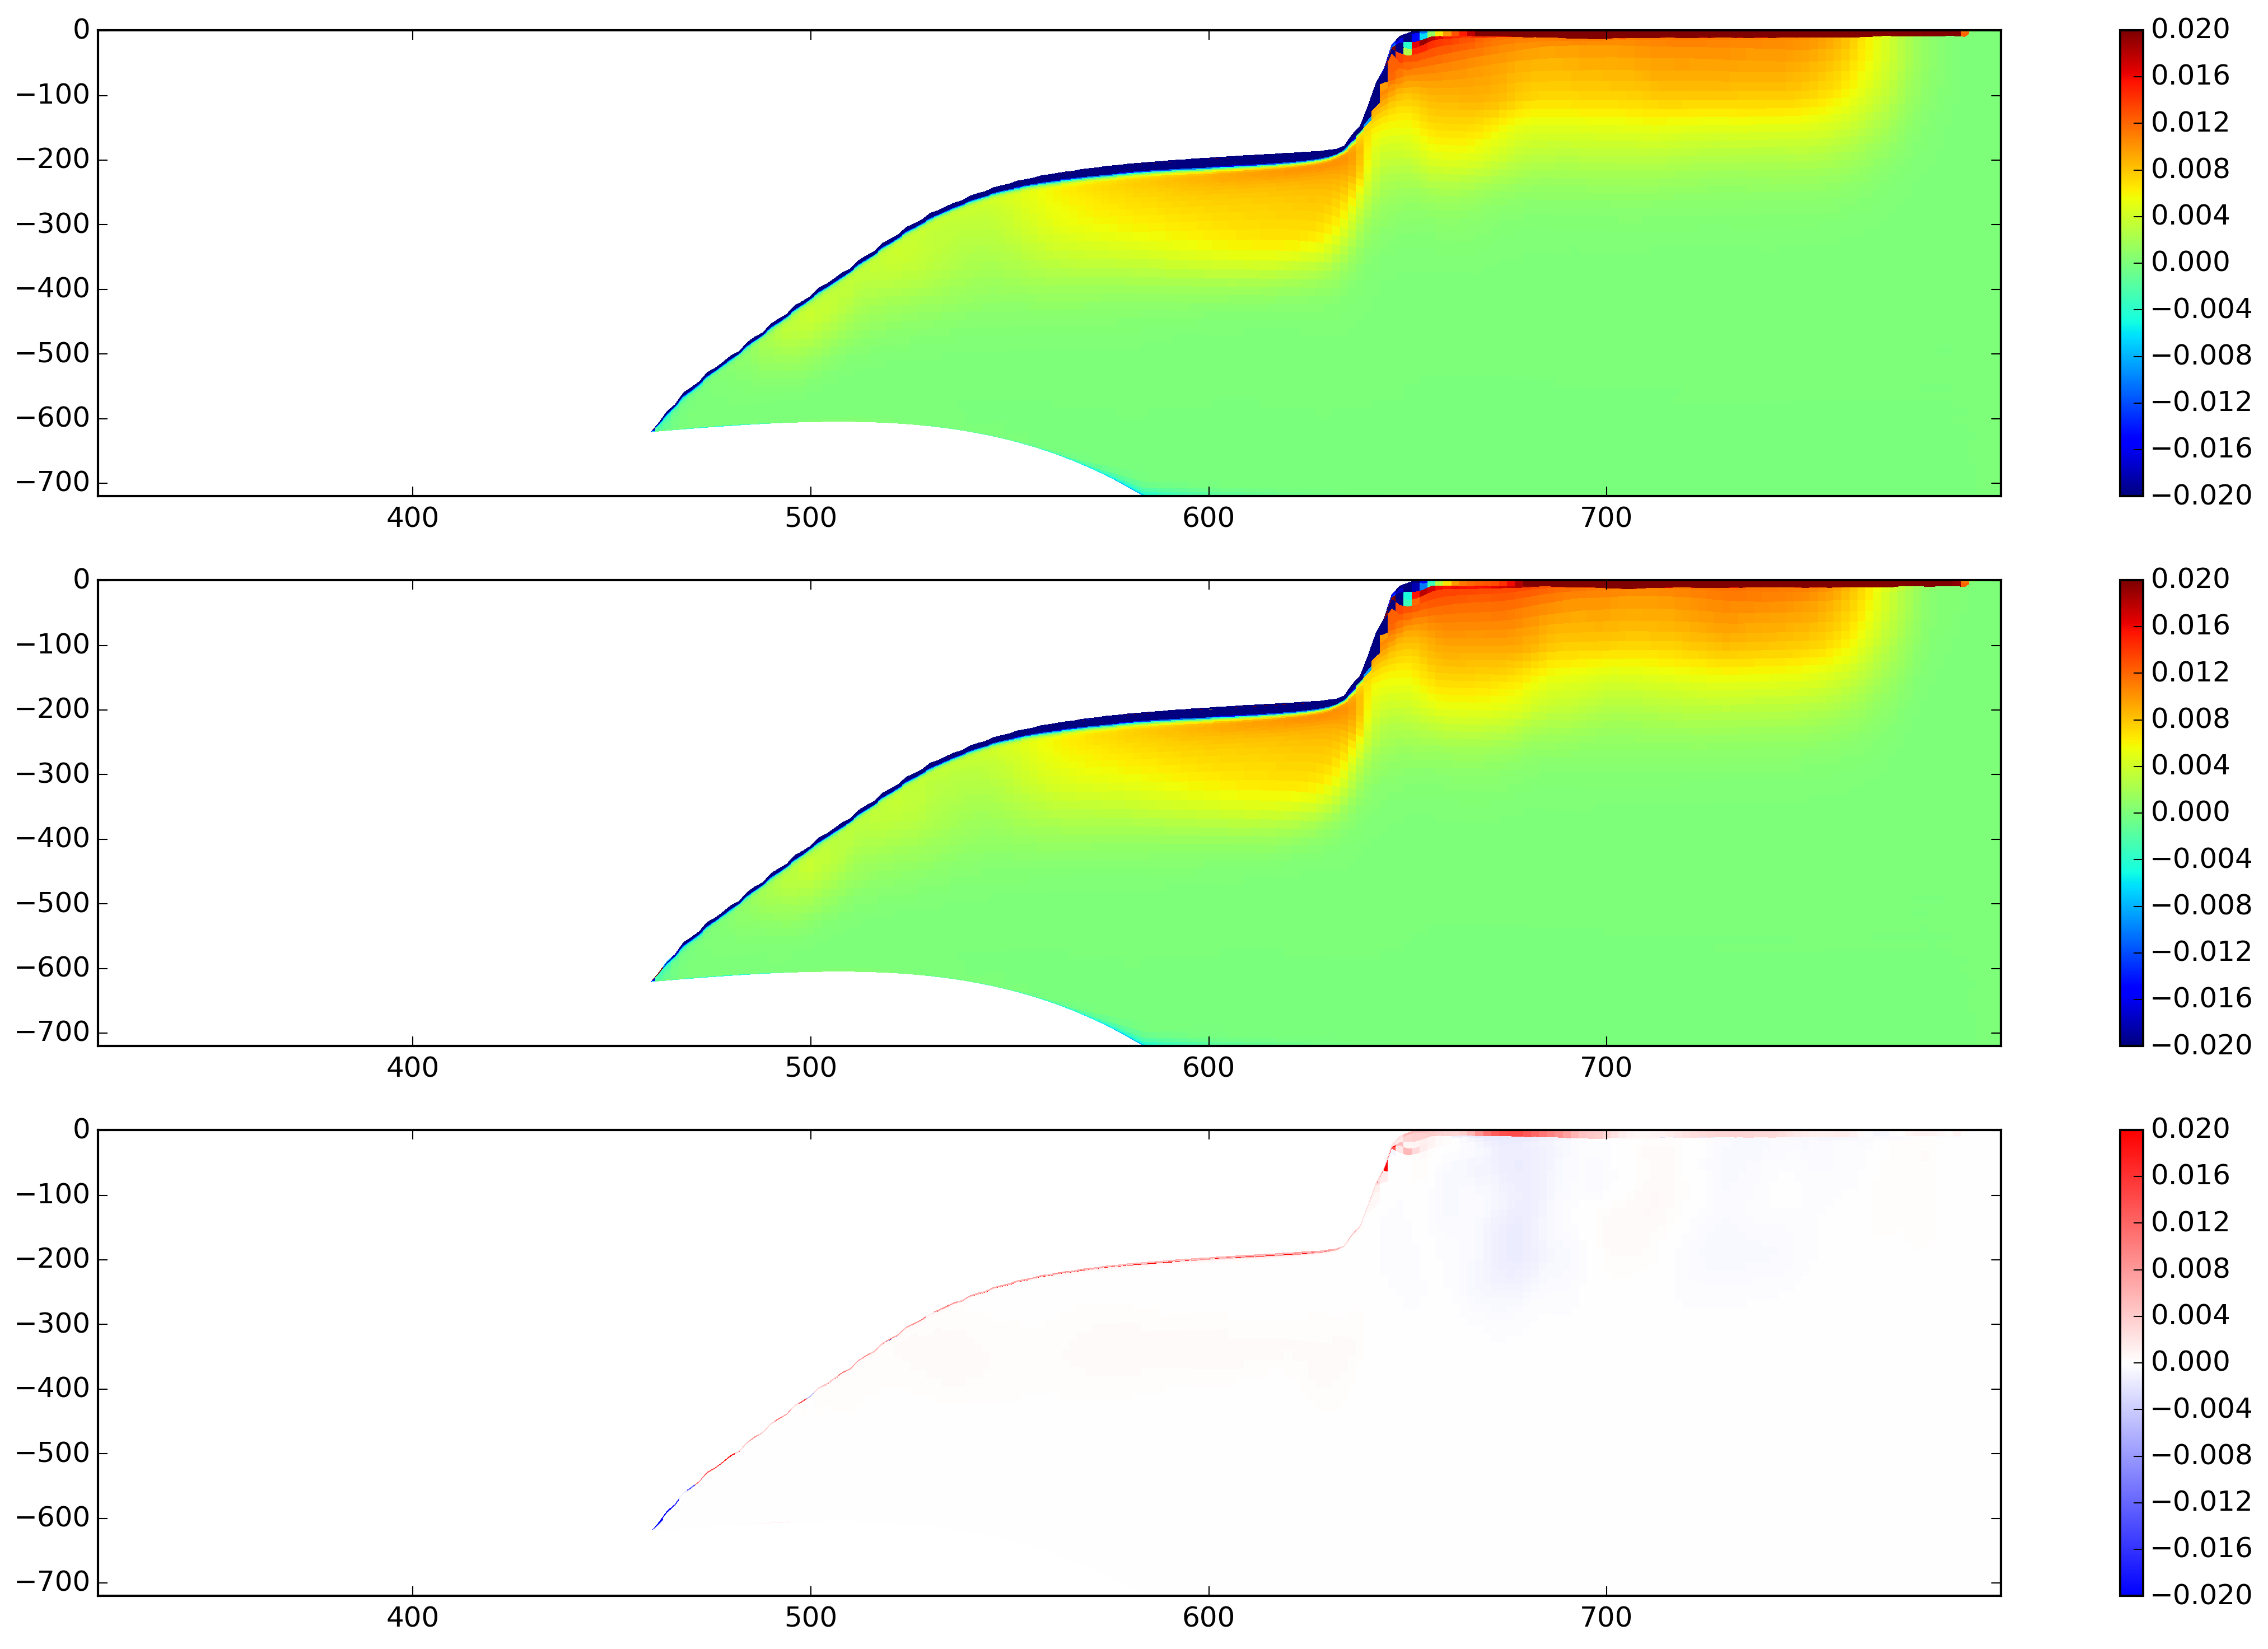
\includegraphics[width=0.99\textwidth]{/Users/alon/Desktop/files/Icebergs_clusters/Towards_Publication/Tech_paper/Github_stuff/Tech-paper/Figures/static_shelf_comparison_salt_layers.png}
\caption{ {Comparison of Eulerian ice-shelf model and Lagrangian ice-shelf model salinity fields.}}
\end{center}
\label{fig:Salt_comparison}
\end{figure}
 \clearpage

 
 



\begin{figure}
\begin{center}
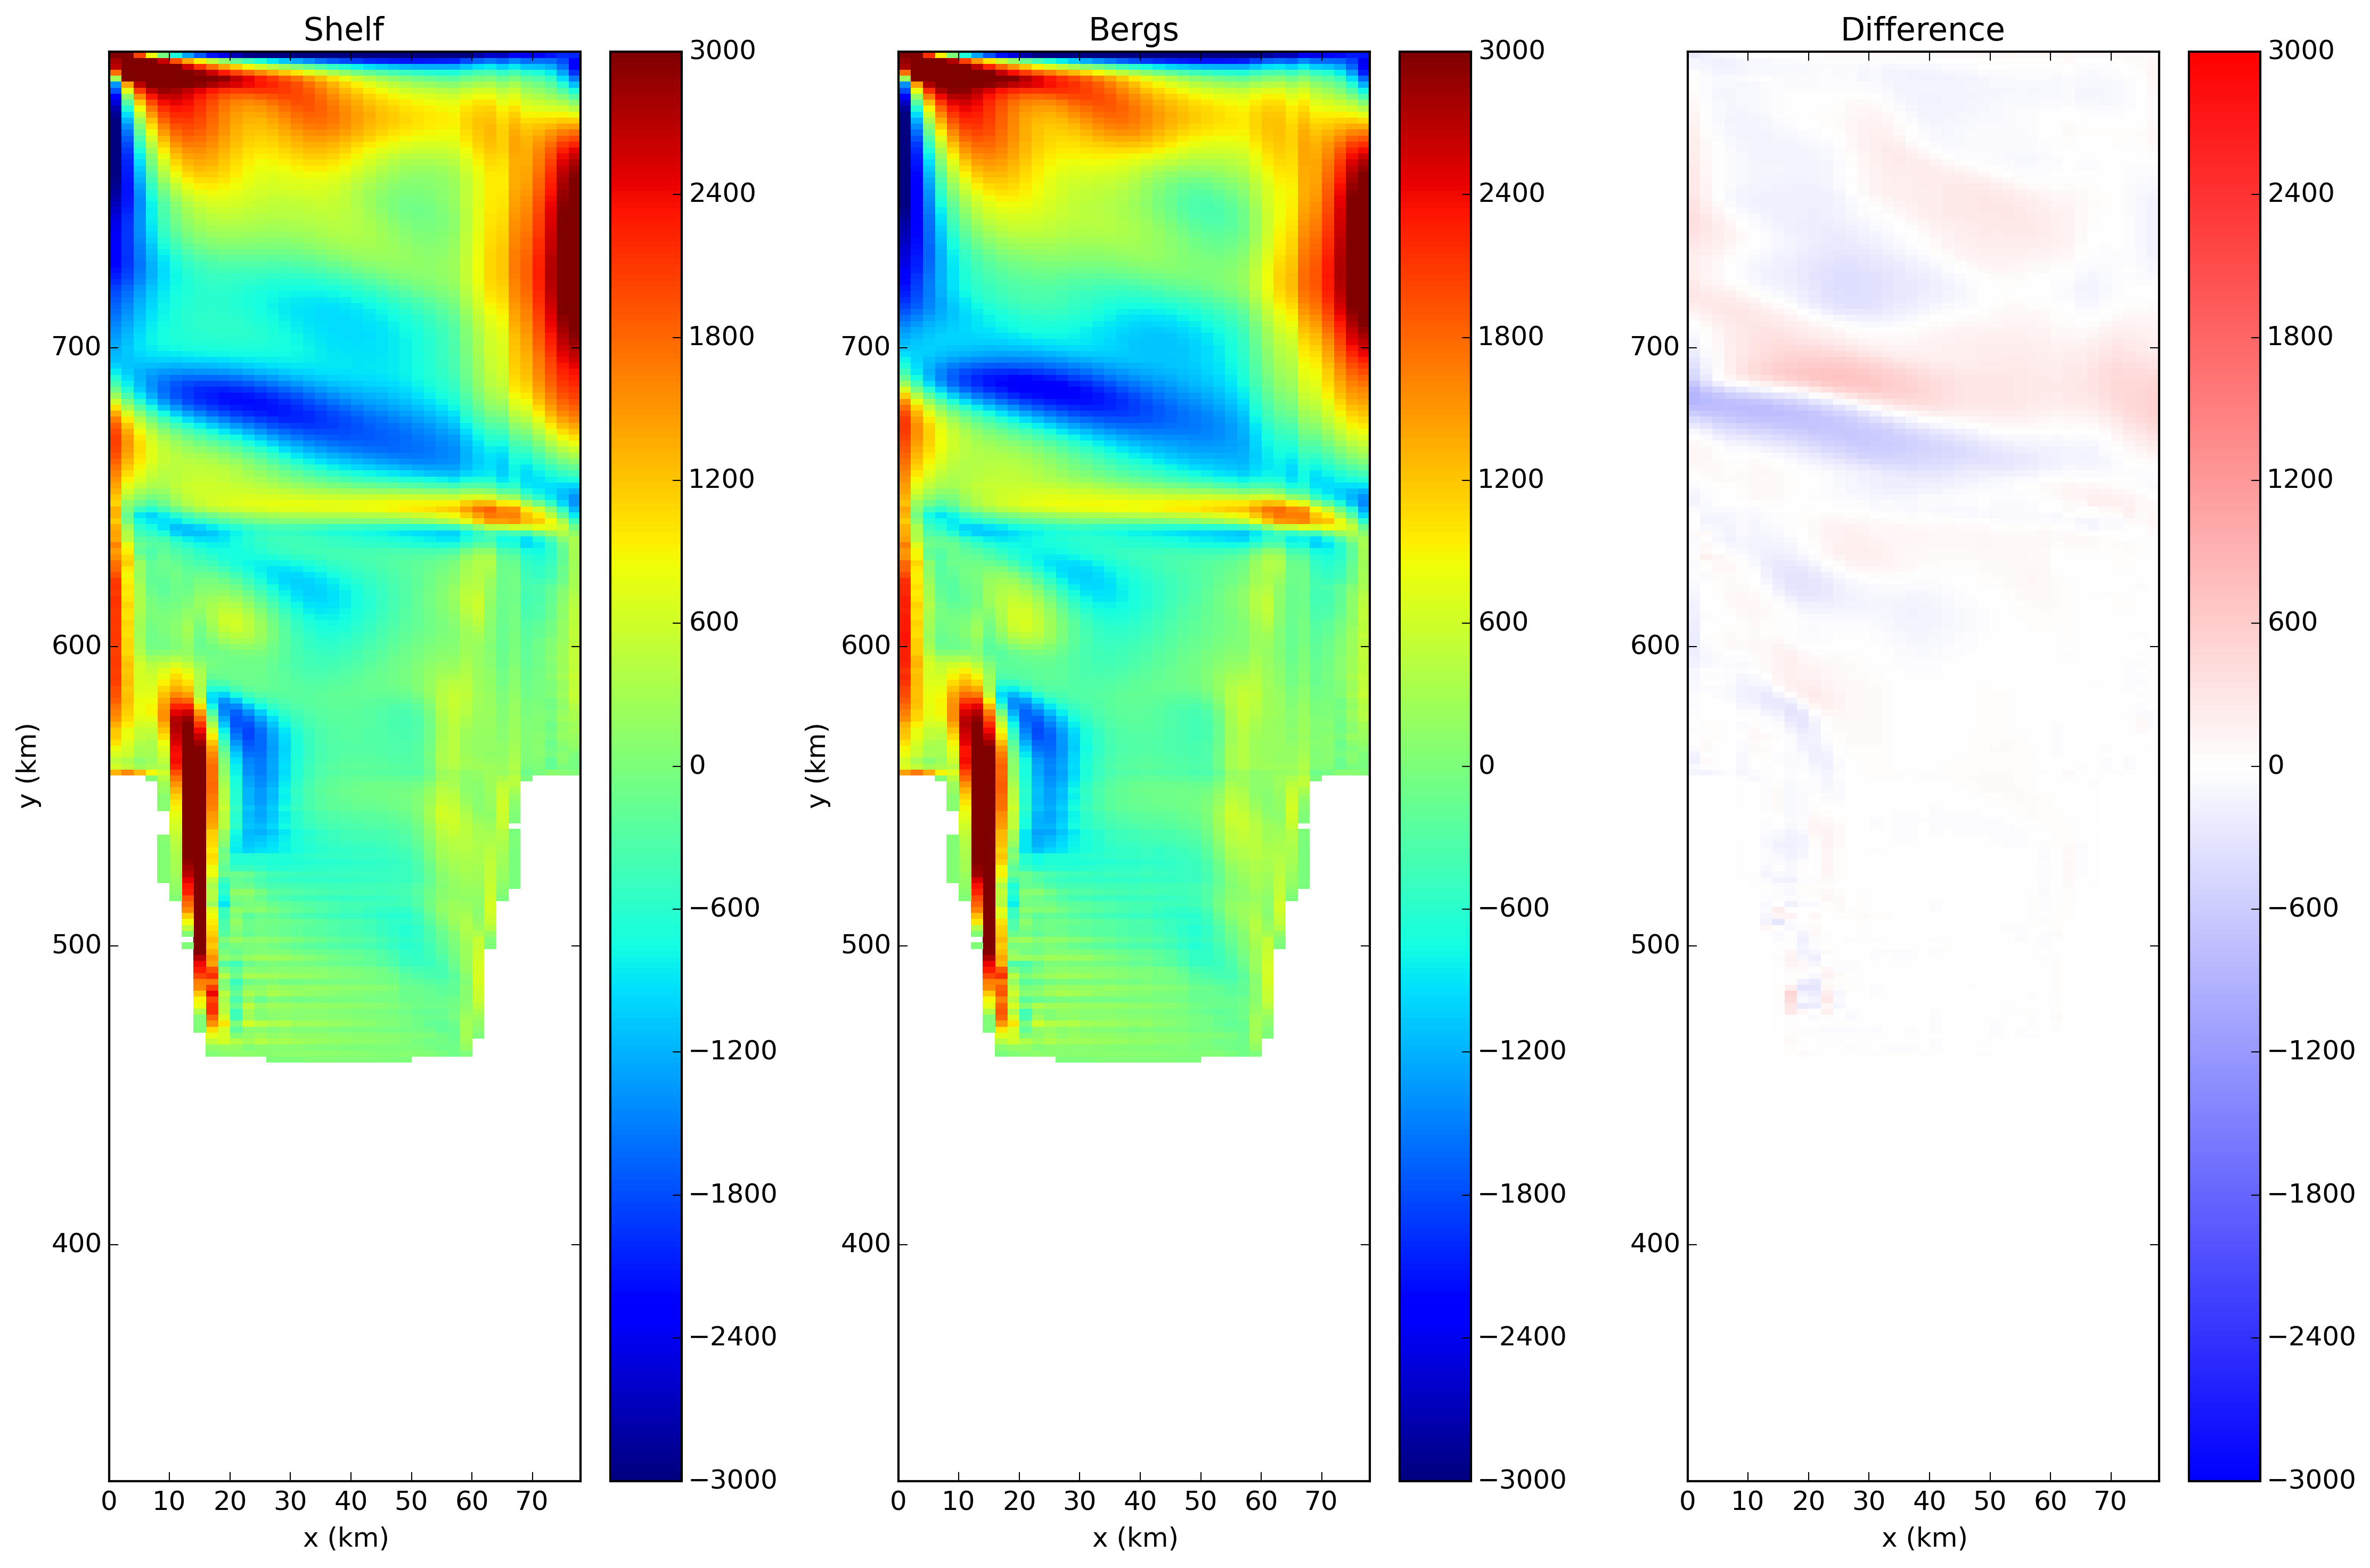
\includegraphics[width=0.99\textwidth]{/Users/alon/Desktop/files/Icebergs_clusters/Towards_Publication/Tech_paper/Github_stuff/Tech-paper/Figures/static_shelf_comparison_barotropic_sf.png}
\caption{ {Layer: Comparison of Eulerian ice-shelf model and Lagrangian ice-shelf model barotropic stream function}}
\end{center}
\label{fig:layer_Bt_comparison}
\end{figure}
 \clearpage   
  
  
  
  
  
  \clearpage


\begin{table}[h!]
\begin{center}
\begin{tabular}{ |c c c c| }
\hline
Parameter & Symbol & Value &  Unit \\
\hline
Domain Length &  $L_{x}$ & 80  & km \\
Domain Width &  $L_{y}$ & 480  & km \\
Horizontal Resolution &  $\Delta x$ & 2  & km \\
Number of vertical layers &  $N_{l}$ & 72  & non-dim\\
Horizontal Viscosity &  $\nu_{H}$ & 6.0 & $\frac{m^{2}}{s}$ \\
Diapycnal Viscosity &  $\nu_{V} $ & $10^{-3}$ & $\frac{m^{2}}{s}$ \\
Horizontal Diffusivity & $ \epsilon_{H}$ & 1.0 & $ \frac{m^{2}}{s}$ \\
Diapycnal Diffusivity &  $\epsilon_{V} $ & $5 \times 10^{-5}$ & $\frac{m^{2}}{s}$ \\
Initial Surface Temperature &  $ T_{t}$& -1.9   & $ ^{o} C$\\
Initial Bottom Temperature &  $ T_{b}$&  1.0  & $ ^{o} C$\\
Initial Surface Salinity &  $ S_{t}$& 33.8   & psu\\
Initial Bottom Salinity &  $ S_{b}$&  34.7  & psu\\
Maximum Ocean depth &  $H_{ocean} $ & 720 & m \\
Relaxation Time of Sponge Layer &  $T_{sponge}$ & 0.1  & days\\
%Background Frictional Velocity Below Ice &  $u^{*}_{bg}$ & 0.0  & 104 \\
%Drag Coefficient Below Ice&  c_{d} & $0.0025$  & (non dim)\\
%Class 9 &  $3.9\times 10^{11}$ & 1659 & 104 \\
Time Step for Static Shelf Experiment & $dt_{Static}$ &  1000  & s\\
Time Step for Iceberg Calving Experiment & $dt_{Calving}$ &  10  & s\\
%Class 1 &  $8.8\times 10^{7}$ & 60  & 0.0026 & 40 & 2000 \\
%Class 2 &  $4.1\times 10^{8}$ & 100 & 0.0072 & 67 & 200\\
%Class 3 &  $3.3\times 10^{9}$ & 200  & 0.029 &133 & 50 \\
%Class 4 &  $1.8\times 10^{10}$& 350 &  0.12 &175  & 20 \\
%Class 5 &  $3.8\times 10^{10}$ & 500  & 0.18 &250 & 10\\
%Class 6 &  $7.5\times 10^{10}$ & 700   & 0.35 &250 & 5\\
%Class 7 &  $1.2\times 10^{11}$ & 900  & 0.56 &250  & 2 \\
%Class 8 &  $2.2\times 10^{11}$ & 1200  & 1.0&250 & 1 \\
%Class 9 &  $3.9\times 10^{11}$ & 1600 & 1.8&250 & 1  \\
%Class 10 & $7.4\times 10^{11}$ &  2200 & 3.5 &250  &1\\
\hline
\end{tabular}
%\caption{Description of the iceberg calving classes used in the model. {\it Mass}, {\it Length}, {\it Area} and {\it Th} refer to the iceberg mass, length, area, and thickness at the time of calving.  {\it Scaling} is the number of icebergs represented by one Lagrangian point particle. The iceberg mass and thickness for each class are the same as those reported in \citet{Gladstone2001}. The iceberg area and length for each class is calculated from the iceberg mass and thickness by assuming that the icebergs are cuboids with a length to width ratio of 1.5, using an iceberg density $\rho_{i}=850$kg/$\textrm{m}^{3}$.}
% Note that the areas of the iceberg classes (calculated from the iceberg lengths and masses given in \citep{Gladstone2001}) are not monotonically increasing.
\label{table:parameters2}
\end{center}
\end{table}

\clearpage

%\begin{figure}
%\begin{center}
%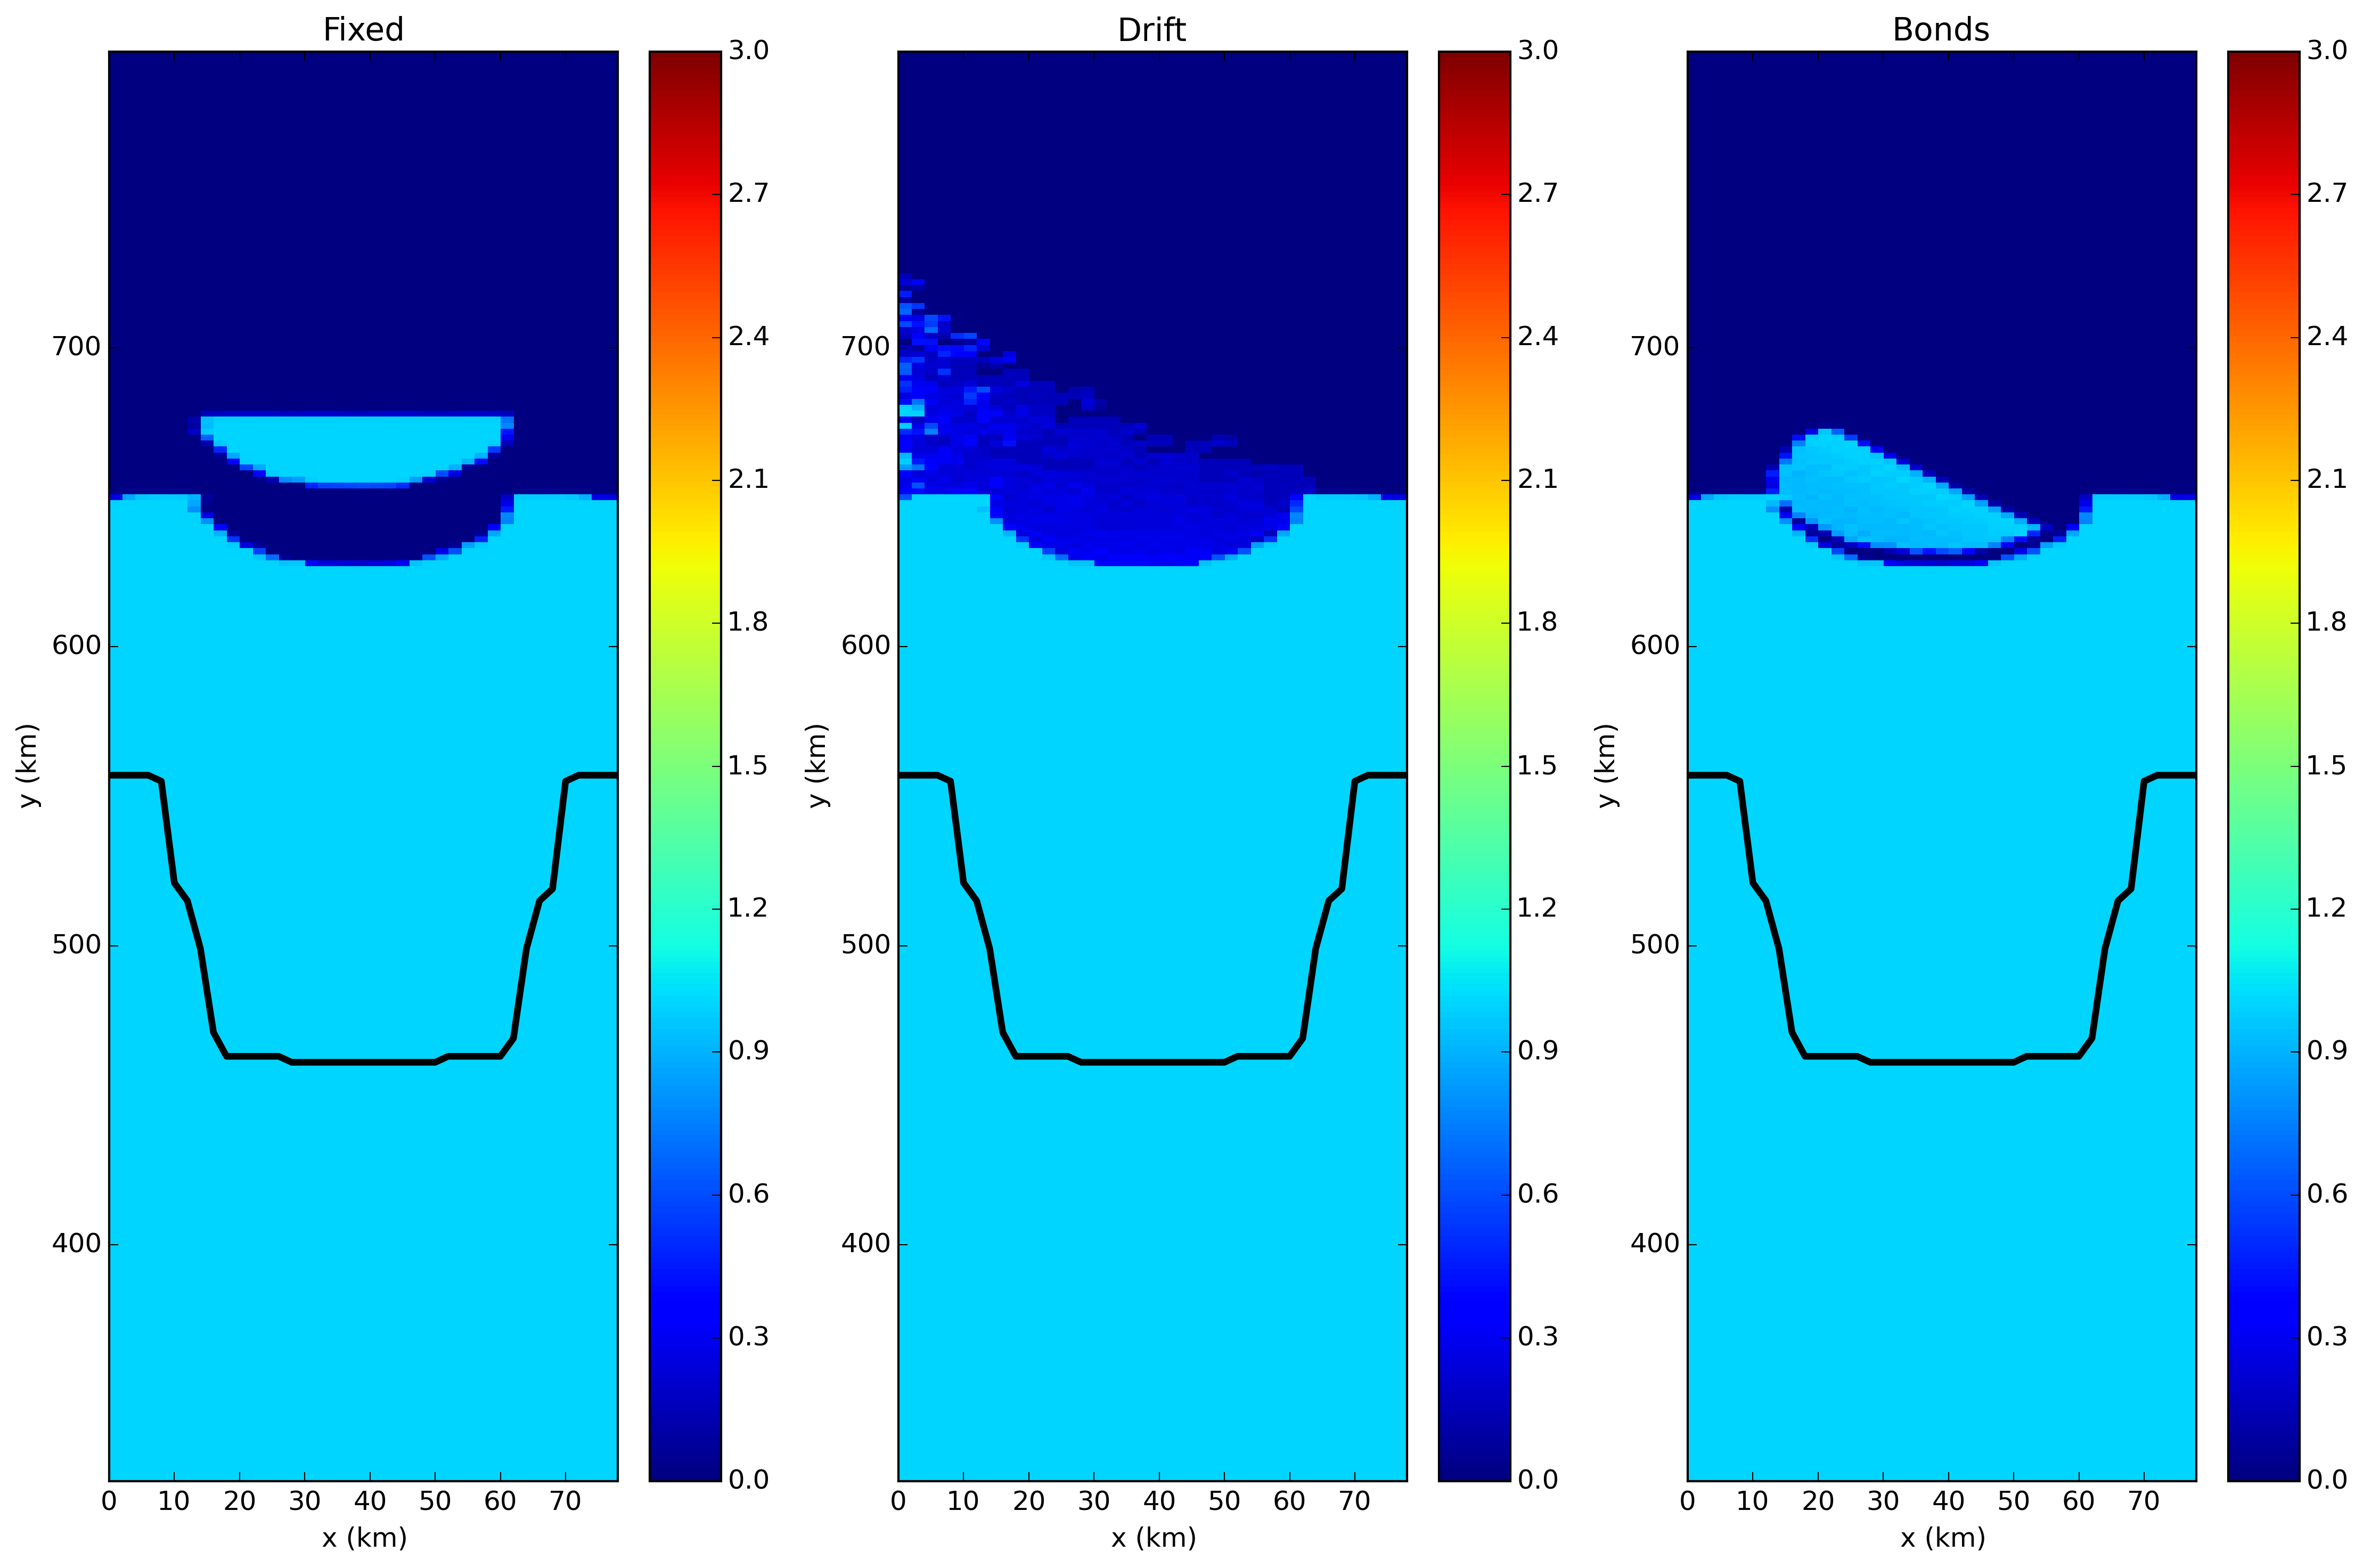
\includegraphics[width=0.99\textwidth]{/Users/alon/Desktop/files/Icebergs_clusters/Towards_Publication/Tech_paper/Github_stuff/Tech-paper/Figures/fixed_drift_bond_spread_area.png}
%\caption{ {Need to update this Figure. Also, I should try using orientation with the Bonds.}}
%\end{center}
%FIgure created by \end{center}
%\label{fig:}
%\end{figure}


% \clearpage

%\begin{figure}
%\begin{center}
%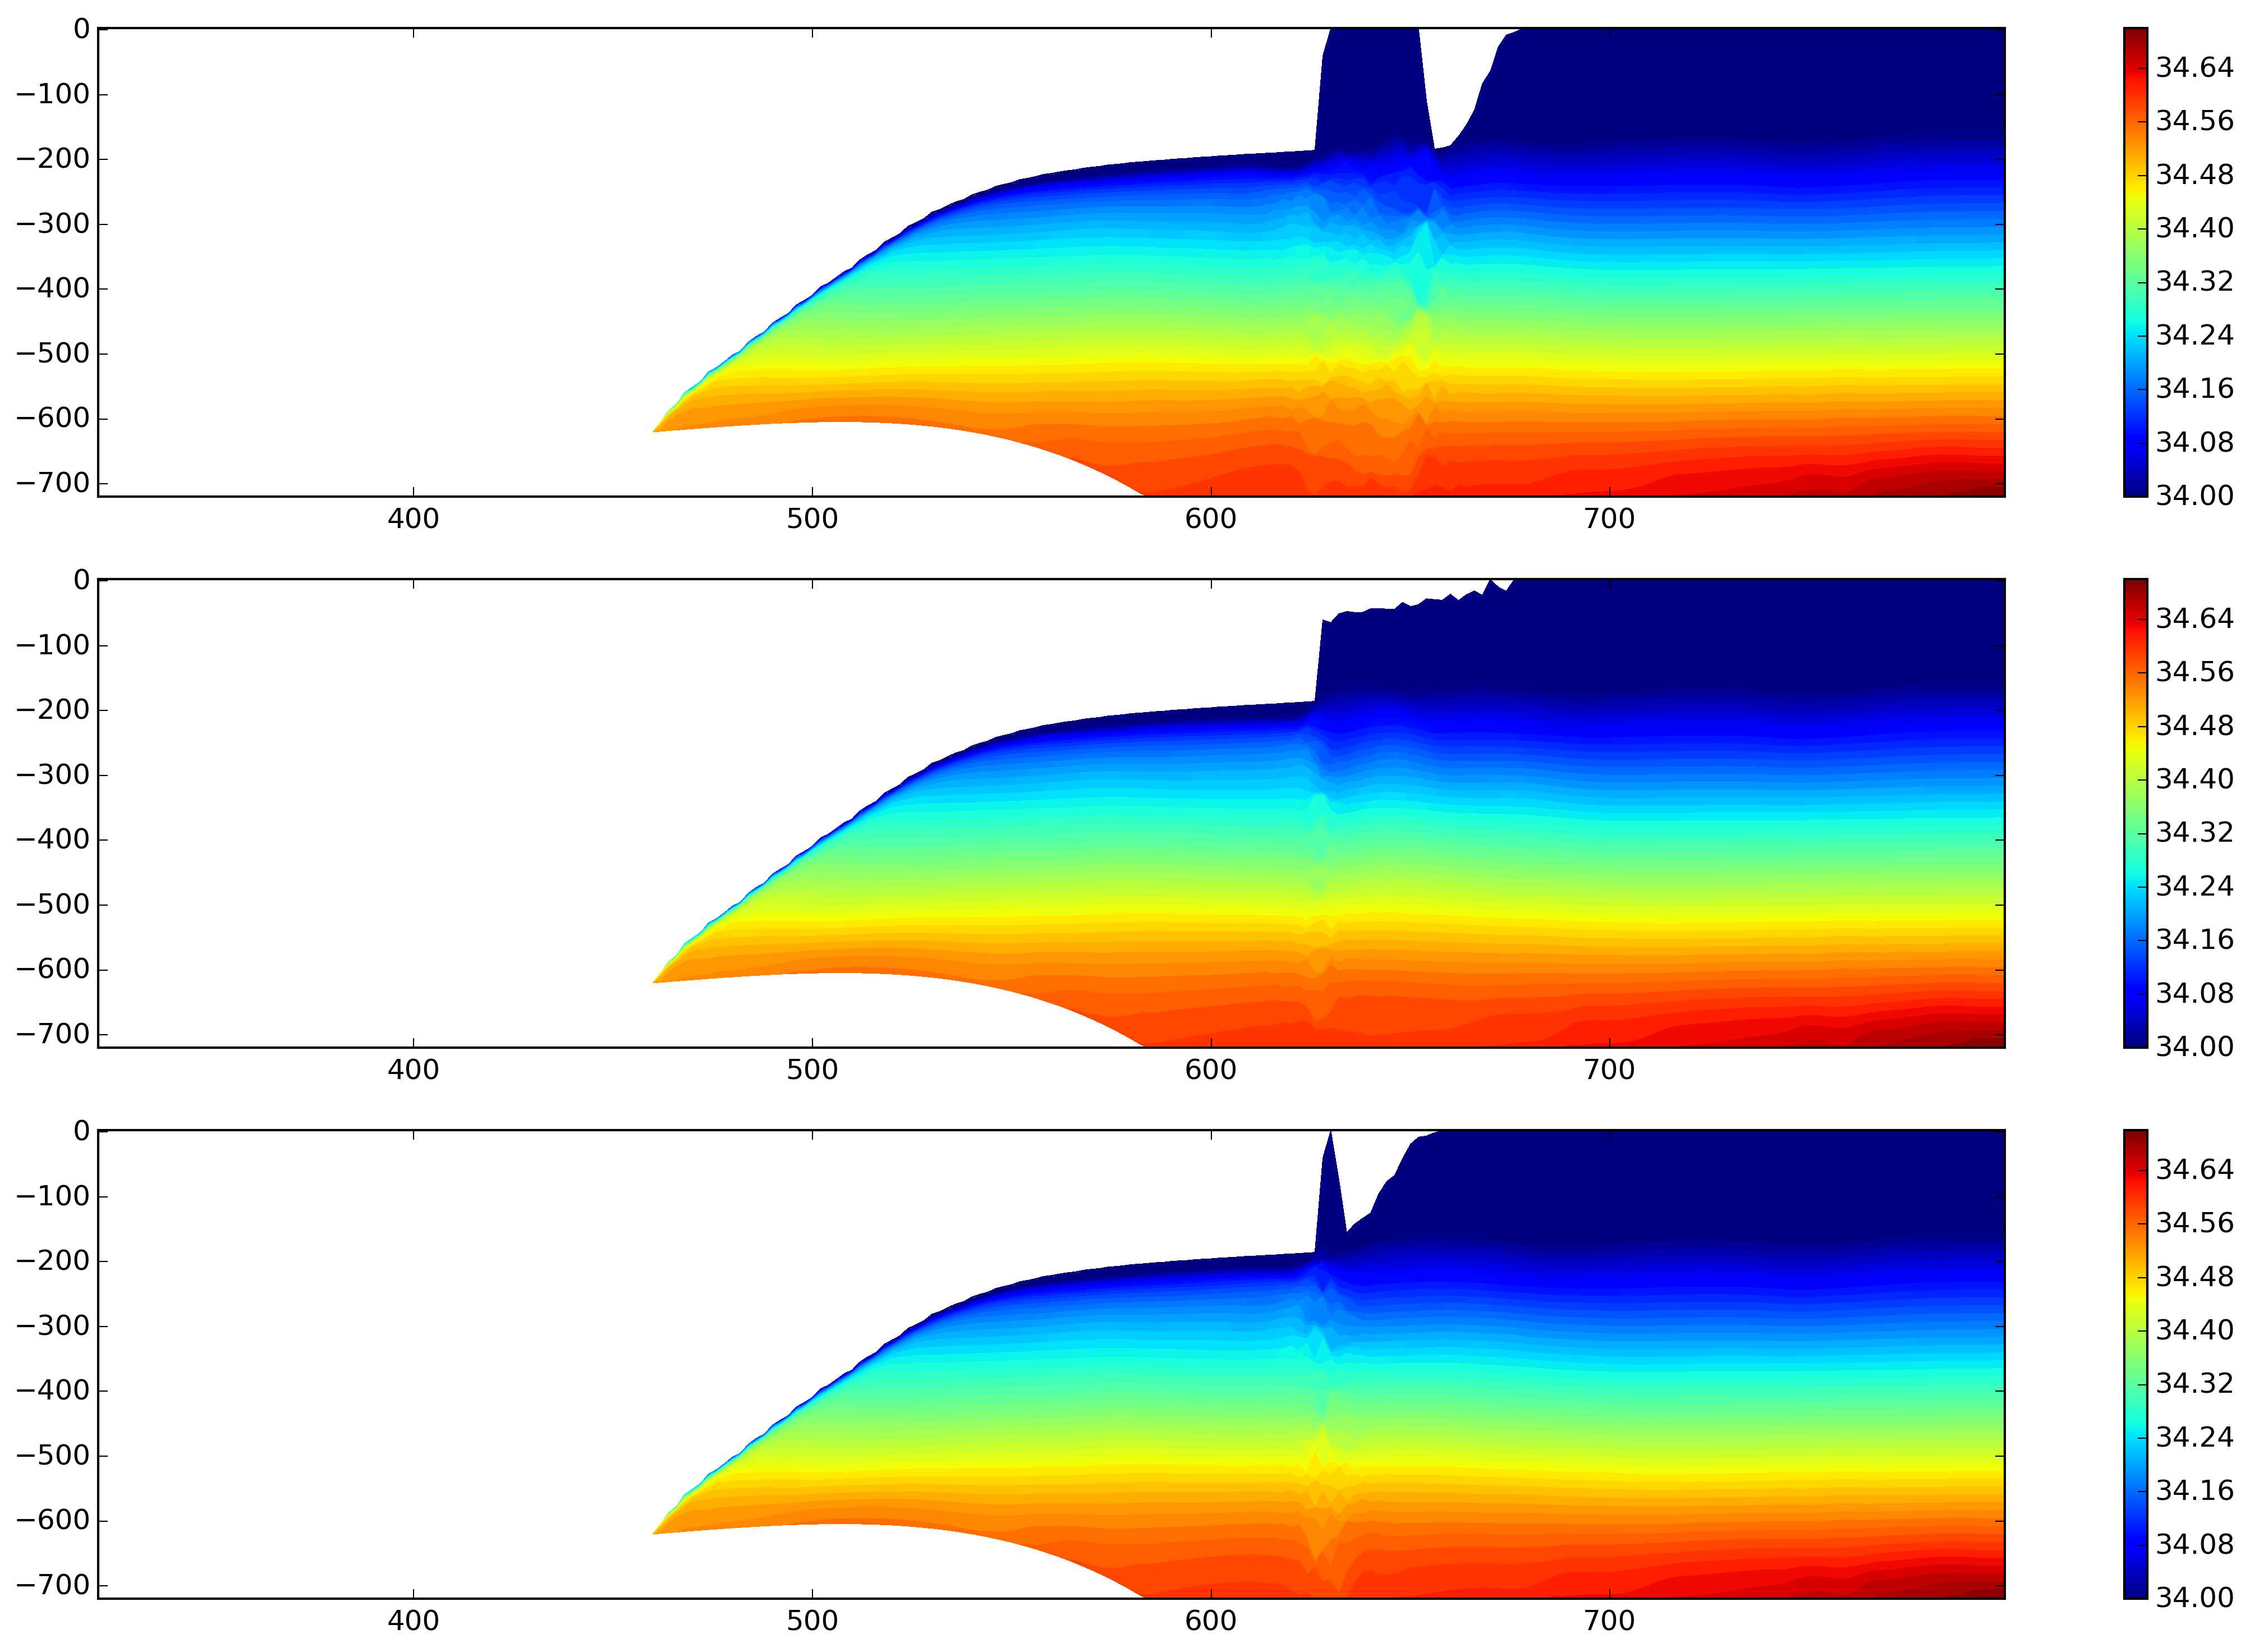
\includegraphics[width=0.99\textwidth]{/Users/alon/Desktop/files/Icebergs_clusters/Towards_Publication/Tech_paper/Github_stuff/Tech-paper/Figures/fixed_drift_bond_salt_layers.png}
%\caption{ {}}
%\end{center}
%FIgure created by \end{center}
%\label{fig:}
%\end{figure}

%\clearpage

%\begin{figure}
%\begin{center}
%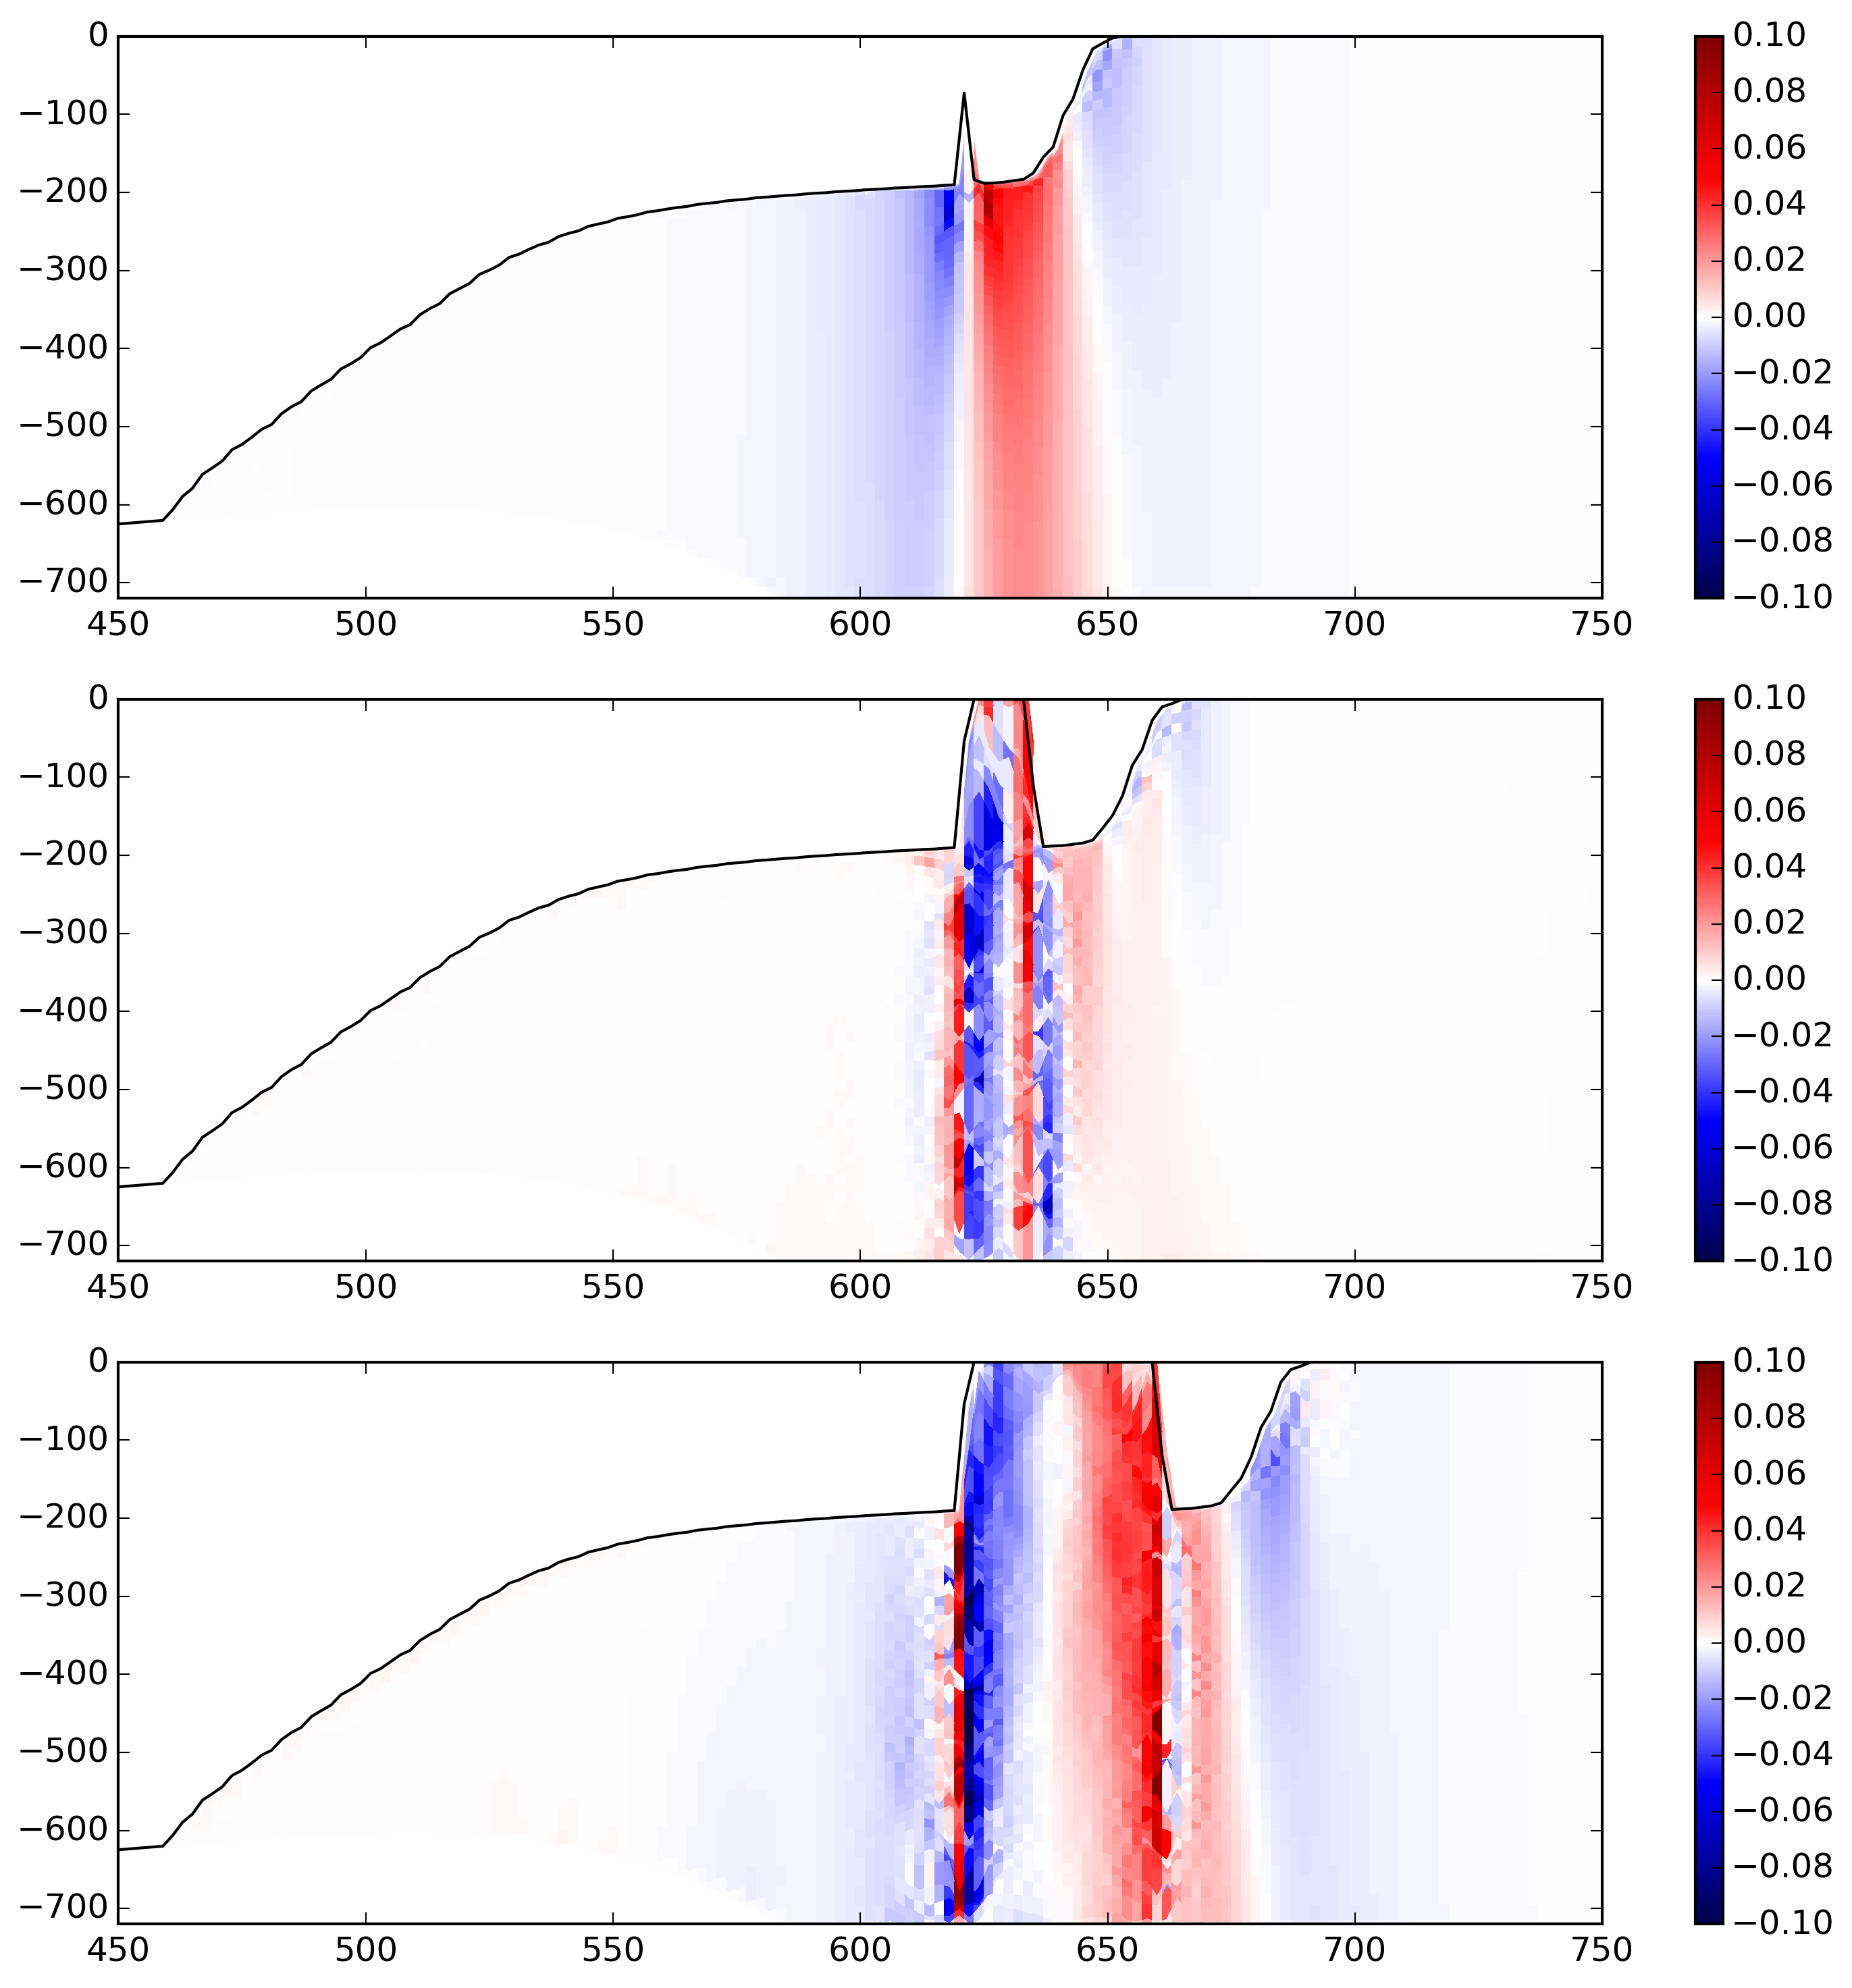
\includegraphics[width=0.99\textwidth]{/Users/alon/Desktop/files/Icebergs_clusters/Towards_Publication/Tech_paper/Github_stuff/Tech-paper/Figures/snapshots_fixed_01_u_layers.png}
%\caption{ {Need to update this Figure. }}
%\end{center}
%FIgure created by \end{center}
%\label{fig:}
%\end{figure}


%\clearpage

%\begin{figure}
%\begin{center}
%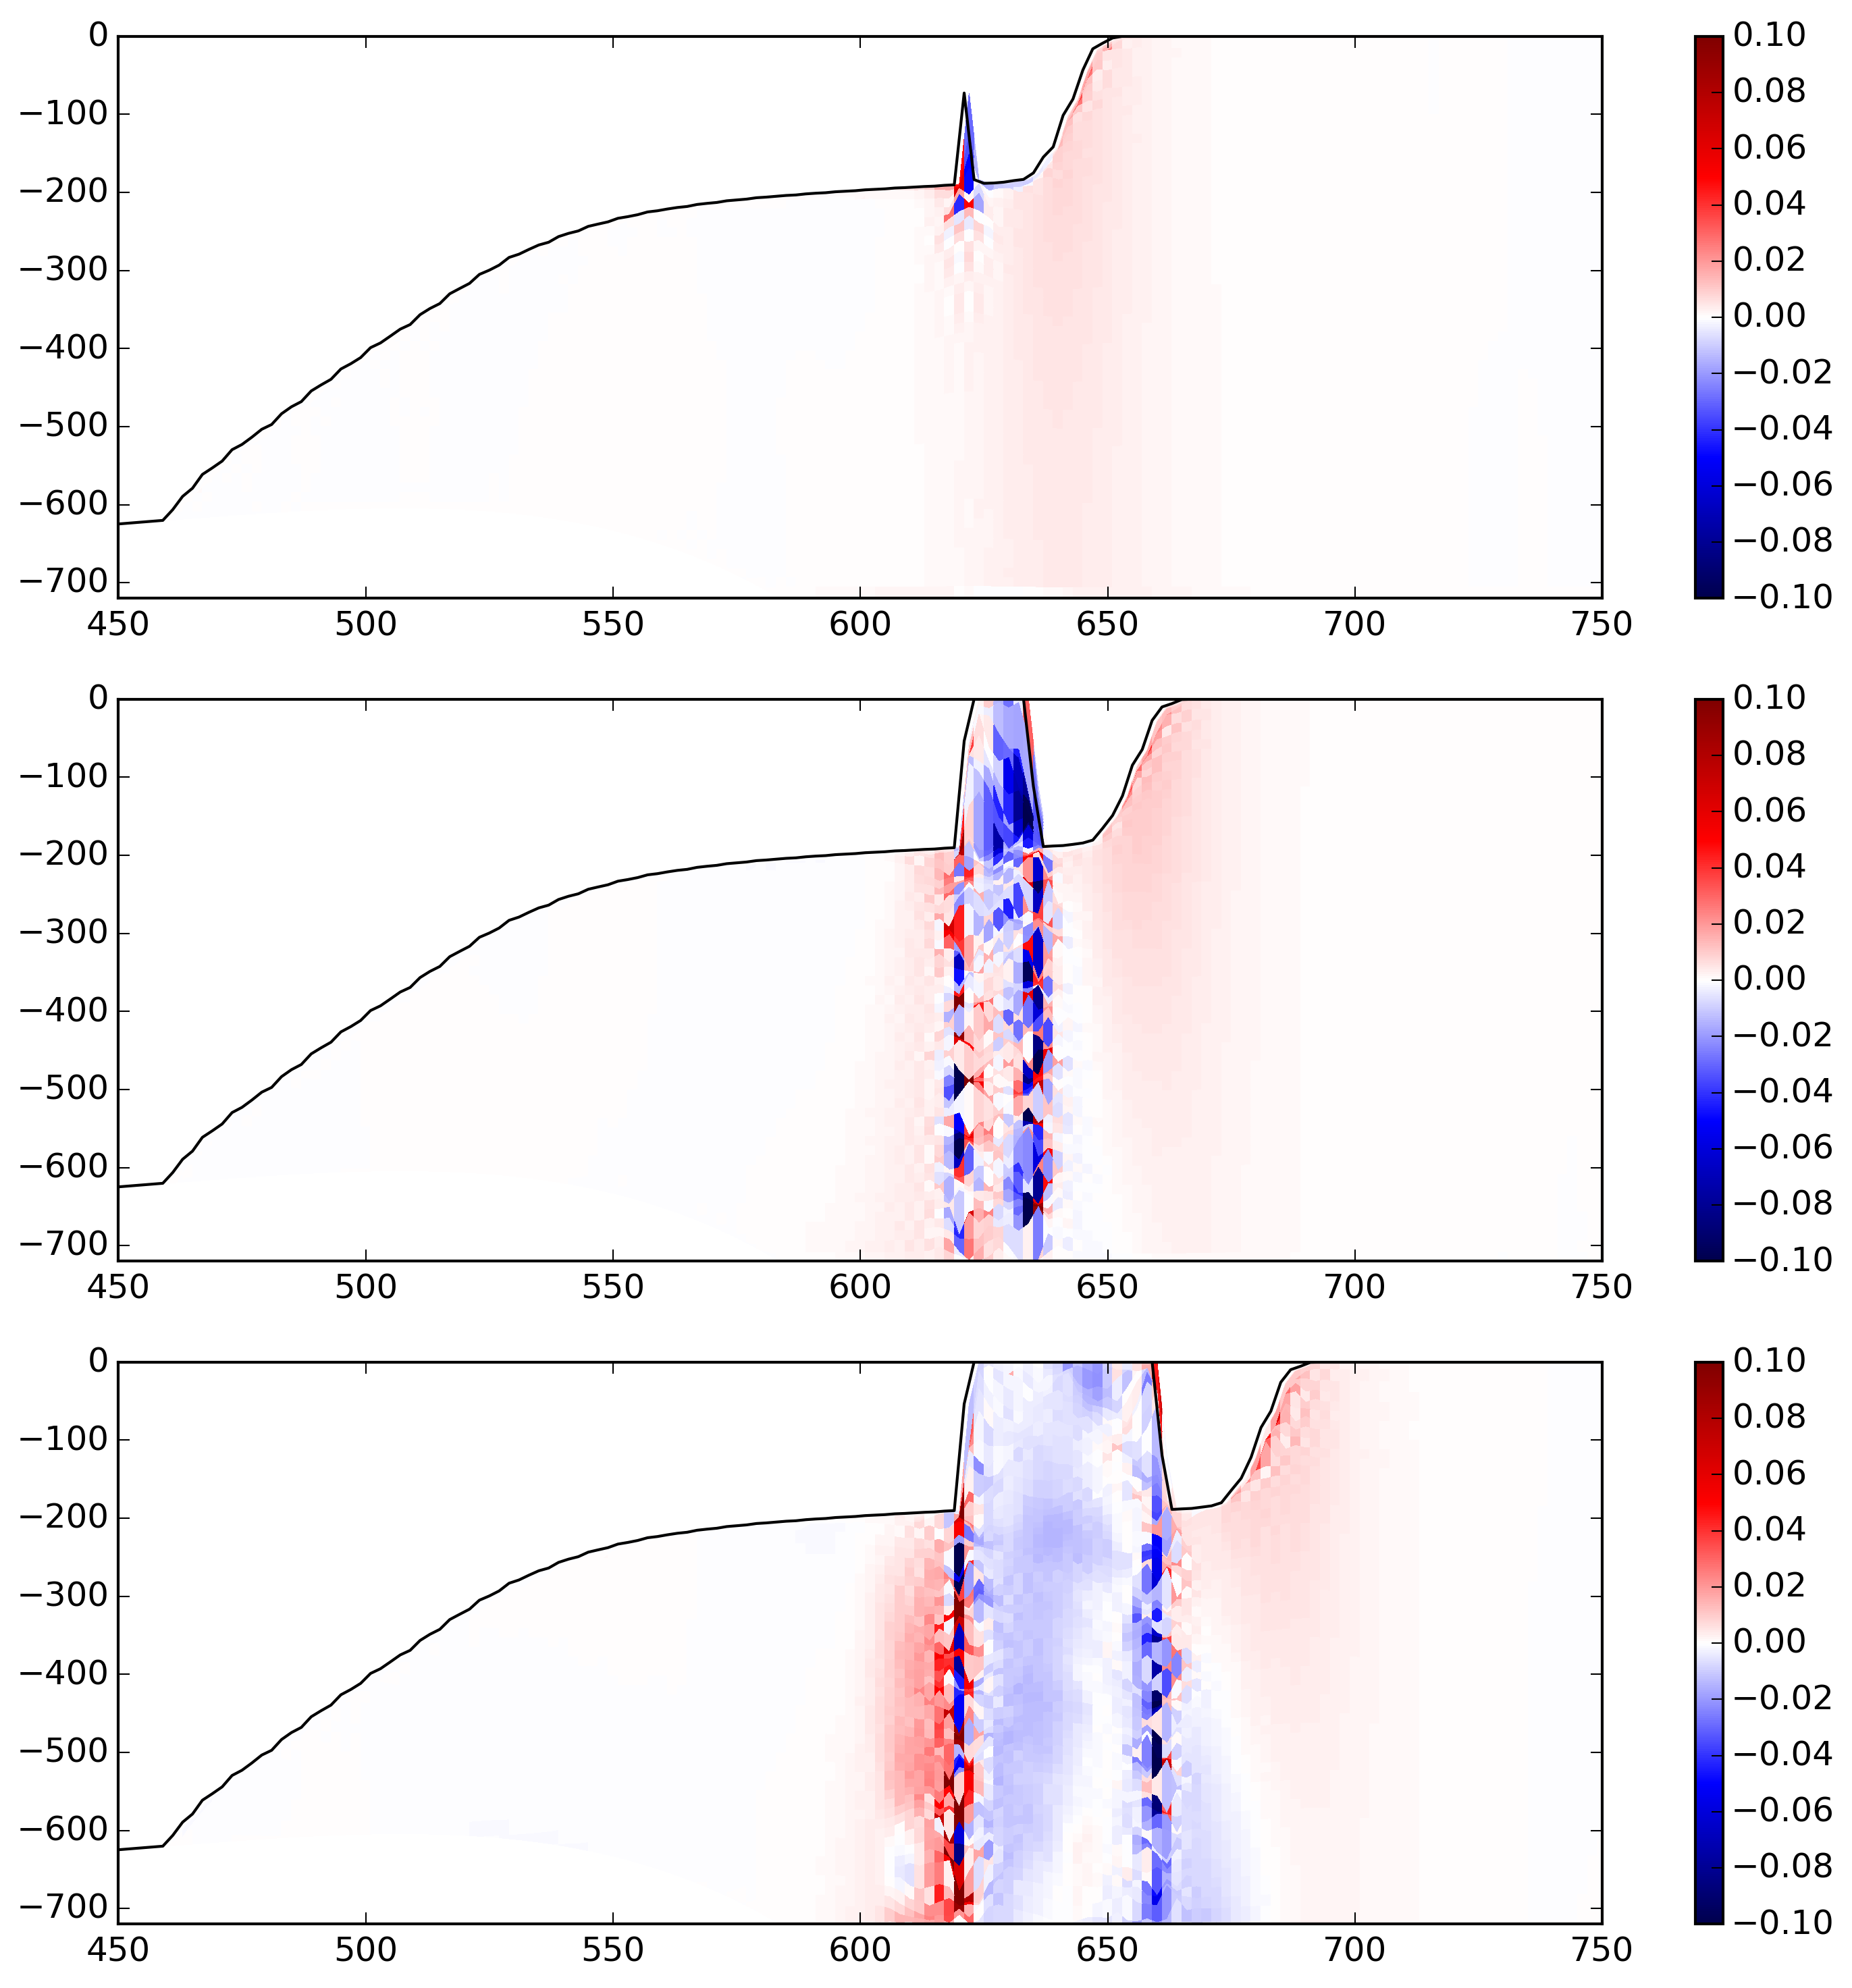
\includegraphics[width=0.99\textwidth]{/Users/alon/Desktop/files/Icebergs_clusters/Towards_Publication/Tech_paper/Github_stuff/Tech-paper/Figures/snapshots_fixed_01_v_layers.png}
%\caption{ {Need to update this Figure. }}
%\end{center}
%FIgure created by \end{center}
%\label{fig:}
%\end{figure}



%%%%%%%%%%%%%%%%%%%%%%%%%%%%%%%%%%%%%%%%%%%%%%%%%%%%%%%%%%%%%%%%%%%%%%%%%%%%%%%%%%%%%
%%%%%%%%%%%%%%%%%%%%%%%%%%%%%%%%%%%%%%%%%%%%%%%%%%%%%%%%%%%%%%%%%%%%%%%%%%%%%%%%%%%%%
%%%%%%%%%%%%%%%%%%%%%%%%%%%%%%%%%%%%%%%%%%%%%%%%%%%%%%%%%%%%%%%%%%%%%%%%%%%%%%%%%%%%%
%%%%%%%%%%%%%%%%%%%%%%%%%%%%%%%%%%%%%%%%%%%%%%%%%%%%%%%%%%%%%%%%%%%%%%%%%%%%%%%%%%%%%
%%%%%%%%%%%%%%%%%%%%%%%%%%%%%%%%%%%%%%%%%%%%%%%%%%%%%%%%%%%%%%%%%%%%%%%%%%%%%%%%%%%%%
%%%%%%%%%%%%%%%%%%%%%%%%%%%%%%%%%%%%%%%%%%%%%%%%%%%%%%%%%%%%%%%%%%%%%%%%%%%%%%%%%%%%%
%%%%%%%%%%%%%%%%%%%%%%%%%%%%%%%%%%%%%%%%%%%%%%%%%%%%%%%%%%%%%%%%%%%%%%%%%%%%%%%%%%%%%
%%%%%%%%%%%%%%%%%%%%%%%%%%%%%%%%%%%%%%%%%%%%%%%%%%%%%%%%%%%%%%%%%%%%%%%%%%%%%%%%%%%%%
%%%%%%%%%%%%%%%%%%%%%%%%%%%%%%%%%%%%%%%%%%%%%%%%%%%%%%%%%%%%%%%%%%%%%%%%%%%%%%%%%%%%%
%%%%%%%%%%%%%%%%%%%%%%%%%%%%%%%%%%%%%%%%%%%%%%%%%%%%%%%%%%%%%%%%%%%%%%%%%%%%%%%%%%%%%
%%%%%%%%%%%%%%%%%%%%%%%%%%%                       Supplementary Figures                   %%%%%%%%%%%%%%%%%%%%%%%%%%%%%%%%%
%%%%%%%%%%%%%%%%%%%%%%%%%%%%%%%%%%%%%%%%%%%%%%%%%%%%%%%%%%%%%%%%%%%%%%%%%%%%%%%%%%%%%
%%%%%%%%%%%%%%%%%%%%%%%%%%%%%%%%%%%%%%%%%%%%%%%%%%%%%%%%%%%%%%%%%%%%%%%%%%%%%%%%%%%%%
%%%%%%%%%%%%%%%%%%%%%%%%%%%%%%%%%%%%%%%%%%%%%%%%%%%%%%%%%%%%%%%%%%%%%%%%%%%%%%%%%%%%%
%%%%%%%%%%%%%%%%%%%%%%%%%%%%%%%%%%%%%%%%%%%%%%%%%%%%%%%%%%%%%%%%%%%%%%%%%%%%%%%%%%%%%
%%%%%%%%%%%%%%%%%%%%%%%%%%%%%%%%%%%%%%%%%%%%%%%%%%%%%%%%%%%%%%%%%%%%%%%%%%%%%%%%%%%%%
%%%%%%%%%%%%%%%%%%%%%%%%%%%%%%%%%%%%%%%%%%%%%%%%%%%%%%%%%%%%%%%%%%%%%%%%%%%%%%%%%%%%%
%%%%%%%%%%%%%%%%%%%%%%%%%%%%%%%%%%%%%%%%%%%%%%%%%%%%%%%%%%%%%%%%%%%%%%%%%%%%%%%%%%%%%
%%%%%%%%%%%%%%%%%%%%%%%%%%%%%%%%%%%%%%%%%%%%%%%%%%%%%%%%%%%%%%%%%%%%%%%%%%%%%%%%%%%%%
%%%%%%%%%%%%%%%%%%%%%%%%%%%%%%%%%%%%%%%%%%%%%%%%%%%%%%%%%%%%%%%%%%%%%%%%%%%%%%%%%%%%%
%%%%%%%%%%%%%%%%%%%%%%%%%%%%%%%%%%%%%%%%%%%%%%%%%%%%%%%%%%%%%%%%%%%%%%%%%%%%%%%%%%%%%
%%%%%%%%%%%%%%%%%%%%%%%%%%%%%%%%%%%%%%%%%%%%%%%%%%%%%%%%%%%%%%%%%%%%%%%%%%%%%%%%%%%%%

\clearpage
\section{Supplementary Figures}
\clearpage

\setcounter{figure}{0}
\renewcommand{\thefigure}{S\arabic{figure}}




  
   
   

 

 \end{document}

%%%%%%%%%%%%%%%%%%%%%%%%%%%%%%%%%%%%%%%%%%%%%%%%%%%%%%%%%%%%%%%

